\documentclass{article}  % Define la clase del documento.

% Paquetes de idioma y codificación
\usepackage[utf8]{inputenc}
\usepackage[T1]{fontenc}
%\usepackage[spanish]{babel}  % Ajusta el idioma del documento a español.
\usepackage{tabularx}  % Permite la creación de tablas con ancho ajustable.

\usepackage{caption}
\usepackage{subcaption}

% Paquete de geometría para configurar márgenes y tamaño de papel
\usepackage[letterpaper, margin=3cm]{geometry}

\usepackage[english]{babel}
\addto\captionsspanish{%
  \renewcommand{\tablename}{Table}%
  \renewcommand{\figurename}{Figure}%
}

% Paquetes de tipografía
\usepackage{mathptmx}    % Usa Times New Roman como fuente.
\usepackage{microtype}   % Mejora la justificación del texto.

% Paquetes para manejo de colores y gráficos
\usepackage{xcolor}      % Define y utiliza colores.
\usepackage{graphicx}    % Permite la inserción de imágenes.
\usepackage{tikz}        % Creación de gráficos vectoriales.

% Configuración de enlaces y referencias cruzadas
\usepackage{hyperref}
\hypersetup{
    colorlinks   = true,
    linkcolor    = darkblue,
    citecolor    = black,
    filecolor    = blue,
    urlcolor     = blue
}

\usepackage{media9} % Permite la inserción de multimedia.

% Paquetes para la mejora visual de tablas y figuras
\usepackage{booktabs}    % Para tablas de alta calidad.
\usepackage{float}       % Controla la posición de figuras y tablas.

% Paquete para la personalización de códigos fuente
\usepackage{listings}
\lstset{
    literate=
    {á}{{\'a}}1 {é}{{\'e}}1 {í}{{\'i}}1 {ó}{{\'o}}1 {ú}{{\'u}}1
    {Á}{{\'A}}1 {É}{{\'E}}1 {Í}{{\'I}}1 {Ó}{{\'O}}1 {Ú}{{\'U}}1
    {ñ}{{\~n}}1 {Ñ}{{\~N}}1 {ü}{{\"u}}1 {Ü}{{\"U}}1,
    backgroundcolor=\color{backcolour},
    commentstyle=\color{codegreen},
    keywordstyle=\color{codepurple},
    numberstyle=\tiny\color{codegray},
    stringstyle=\color{red},
    basicstyle=\ttfamily\small,
    breakatwhitespace=false,
    breaklines=true,
    captionpos=b,
    keepspaces=true,
    numbers=left,
    numbersep=5pt,
    showspaces=false,
    showstringspaces=false,
    showtabs=false,
    tabsize=2,
    language=TeX,
    morecomment=[l]\#,
    frame=single,
    rulecolor=\color{black}
}

% Definición de colores al estilo Visual Studio Code
\definecolor{darkblue}{rgb}{0.0, 0.0, 0.55}  % Enlaces
\definecolor{codegreen}{rgb}{0.25, 0.49, 0.48}  % Comentarios
\definecolor{codegray}{rgb}{0.5, 0.5, 0.5}  % Números y anotaciones
\definecolor{codepurple}{rgb}{0.58, 0, 0.82}  % Palabras clave
\definecolor{backcolour}{rgb}{0.95, 0.95, 0.92}  % Fondo de código

% Configuraciones de párrafo y matemáticas
\usepackage{amsmath}
\usepackage{parskip}    % Espaciado entre párrafos.
\usepackage{ragged2e}   % Justificación mejorada.
\usepackage{multicol}

% Configuración de secciones y encabezados
\usepackage{titlesec}
\titleclass{\part}{top} % Make part like a class
\titleformat{\part}[display]
  {\normalfont\huge\bfseries\centering}{\thepart}{40pt}{\Huge}
\titlespacing*{\part}{0pt}{-60pt}{10pt}
\titleformat{\part}
  {\normalfont\huge\bfseries}{}{0pt}{}

% Asegúrate de usar esto para mantener el estilo en las páginas de las partes
\titleformat{\part}[display]
  {\normalfont\huge\bfseries}{}{0pt}{}
  [\thispagestyle{fancy}] % Aplica el estilo fancy a las páginas de las partes

% Configuración de encabezados y pies de página personalizados
\usepackage{fancyhdr}
\pagestyle{fancy}
\fancyhf{}
\fancyhead[L]{\raisebox{0.20cm}{\textbf{Dynamics of structures}}}
\fancyhead[R]{\raisebox{0.1cm}{
\includegraphics[width=0.25\linewidth]{LOGO_UNIVERSIDAD.jpg}}}
\fancyhead[C]{\rule{\textwidth}{0.6pt}}
\fancyfoot[C]{\rule{\textwidth}{0.6pt}}
\fancyfoot[R]{\raisebox{-1.5\baselineskip}{\thepage}}
\renewcommand{\headrulewidth}{0pt}
\renewcommand{\footrulewidth}{0pt}

% Configuración avanzada de geometría
\geometry{
  top=3.5cm, % Aumenta el espacio en la parte superior para subir el encabezado
  bottom=2.5cm,
  headheight=2.5cm % Aumenta la altura del encabezado si es necesario
}

% Configuracion de bibliografia
\usepackage{natbib}
\bibliographystyle{unsrtnat}  % Puedes cambiarlo por `unsrtnat`, `abbrvnat`, etc.

\begin{document}
%----------------------------------------------------------------------------------------
% PORTADA
%----------------------------------------------------------------------------------------
\begin{titlepage}%Inicio de la carátula, solo modificar los datos necesarios
\newcommand{\HRule}{\rule{\linewidth}{0.5mm}} 
\center 
%----------------------------------------------------------------------------------------
%	ENCABEZADO
%----------------------------------------------------------------------------------------

\includegraphics[width=10cm]{LOGO_UNIVERSIDAD.jpg}\\ % Si esta plantilla se copio correctamente, va a llevar la imagen del logo de la facultad.OBS: Es necesario incluir el paquete: graphicx
\vspace{3cm}
%----------------------------------------------------------------------------------------
%	SECCION DEL TITULO
%----------------------------------------------------------------------------------------
\HRule \\[0.4cm]
{ \huge \bfseries Dynamics of structures}\\[0.4cm] % Titulo del documento
{ \huge \bfseries Laboratory 1: Single Degree of Freedom System}\\[0.4cm] % Titulo del documento
\HRule \\[1.5cm]
 \vspace{5cm}
%----------------------------------------------------------------------------------------
%	SECCION DEL AUTOR
%----------------------------------------------------------------------------------------
\begin{flushright}
  { \textbf{Professor:}\\
  Francisco Hernandez\\
  \textbf{Assistance:}\\
  Gastón Parra\\
  \textbf{Students:} \\
  Bernardo Caprile\\
  Pedro Valenzuela\\
  Felipe Vicencio\\
  Lukas Wolff\\
}
\end{flushright}
\vspace{1cm}
%----------------------------------------------------------------------------------------
%	SECCION DE LA FECHA
%----------------------------------------------------------------------------------------
{\large \textbf{\today}}\\[2cm] % El comando \today coloca la fecha del dia, y esto se actualiza con cada compilacion, en caso de querer tener una fecha estatica, reemplazar el \today por la fecha deseada
\end{titlepage}

\newpage
\thispagestyle{empty} % Deshabilita el número de página en la página del índice

%----------------------------------------------------------------------------------------
%  INDICE
%----------------------------------------------------------------------------------------
%\newpage
%\thispagestyle{empty} % Deshabilita el número de página en la página del índice
%\tableofcontents
%\thispagestyle{plain} % Deshabilita el encabezado en la página del índice
%\thispagestyle{empty} % Deshabilita el número de página en la página del índice
%\newpage

%\newpage
%\thispagestyle{empty}
%\listoffigures 
%\thispagestyle{plain} % Deshabilita el encabezado en la página del índice %
%\thispagestyle{empty}
\newpage
%----------------------------------------------------------------------------------------
%ACÁ EMPIEZA EL INFORME
\setcounter{page}{1}
%----------------------------------------------------------------------------------------

\section{Introduction}
To understand the dynamic behavior of complex structures with multiple degrees of freedom, it is essential to first study single degree of freedom (SDOF) systems. These simplified models serve as the foundation for analyzing structural response under dynamic loading. In this laboratory experiment, we aim to determine the natural period and damping ratio of an SDOF system using various experimental methods. This includes performing a pull-back test and applying the logarithmic decrement technique to estimate damping characteristics. Additionally, the system is subjected to harmonic base excitation to identify its natural frequency and evaluate resonance behavior. The results obtained experimentally are then compared to those derived from an analytical model, providing insight into the accuracy and limitations of both approaches. This foundational knowledge is critical for the design and analysis of real-world engineering structures subjected to dynamic forces.


\begin{figure}[h]
  \centering
  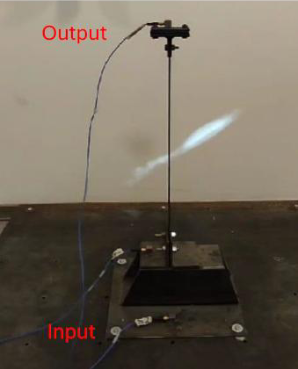
\includegraphics[width=0.5\textwidth]{GRAFICOS/SDOF_picture.PNG}
  \caption{Single Degree of Freedom System.}
  \label{fig:sdof}
\end{figure}
  
The experimental structure used to model the single degree of freedom (SDOF) system consists of a vertical flexible rod rigidly fixed at its base. At the top of the rod, a small mass is attached, allowing for lateral motion when the system is excited. The input motion is applied at the base (as indicated by the “Input” label in the figure), while the output is measured at the top mass using a acceleration sensor (labeled “Output”). This setup simulates the behavior of an idealized SDOF system by allowing one mode of vibration in the lateral direction, the mass, the flexural stiffness of the rod, and the system's inherent damping. It is important to note that, there will be 2 systems analyzed in this laboratory, one without damping (system 1) and one with damping (system 2). The system with damping will have a toothbrush as a damper, while the system without damping will not. 

For more details of the programming, analysis and results, you can visit the files at: \href{https://github.com/LukasWolff2002/LAB_1_DYNAMICS}{GitHub Repository}.



\newpage

\section{Theoretical Background}

\subsection{Natural Frequency}
The natural frequency of a system is the rate at which the body oscillates when it is disturbed without any damping or external forces acting on it. This parameter is crucial in understanding the dynamic behavior of structures, as it determines how the system will respond to external excitations. The natural frequency can be calculated using the following formula:
\begin{equation}
\omega_n = \sqrt{\frac{k}{m}}
\end{equation}
Where:
\begin{itemize}
  \item $\omega_n$ = natural frequency (rad/s)
  \item $k$ = stiffness of the system (N/m)
  \item $m$ = mass of the system (kg)
\end{itemize}

One of the important aspects of the natural frequency is that it is inversely proportional to the mass of the system. This means that as the mass increases, the natural frequency decreases, and vice versa. This relationship is crucial in designing structures to ensure they can withstand dynamic loads without resonating at their natural frequency.

\subsection{Damping Ratio}
The damping ratio is a parameter that has the effect of reducing the oscillations of a system over time. In physical systems, damping is caused by energy dissipation mechanisms such as friction, air resistance or dampers. The damping ratio is defined as the ratio of the actual damping to the critical damping, and it can be calculated using the following formula:
\begin{equation}
\beta = \frac{c}{2\sqrt{mk}}
\end{equation}
Where:
\begin{itemize}
  \item $\beta$ = damping ratio (dimensionless)
  \item $c$ = damping coefficient (N.s/m)
  \item $k$ = stiffness of the system (N/m)
  \item $m$ = mass of the system (kg)
\end{itemize}

\subsection{Logarithmic Decrement}
The logarithmic decrement is a measure of the rate at which the amplitude of oscillations decreases over time in a damped system. It is defined as the natural logarithm of the ratio of two successive amplitudes, and it can be calculated using the following formula:

\begin{equation}
\delta = \frac{1}{n} \ln \left( \frac{x_0}{x_n} \right)
\end{equation}
Where:
\begin{itemize}
  \item $\delta$ = logarithmic decrement (dimensionless)
  \item $x_0$ = amplitude of the first oscillation (m)
  \item $x_n$ = amplitude of the n-th oscillation (m)
  \item $n$ = number of oscillations (dimensionless)
\end{itemize}

With this parameter, we can determine the damping ratio of the system using the following formula:

\begin{equation}
\beta = \frac{\delta}{\sqrt{4\pi^2 + \delta^2}}
\label{eq:log_dec}
\end{equation}
Where:
\begin{itemize}
  \item $\delta$ = logarithmic decrement (dimensionless)
  \item $\beta$ = damping ratio (dimensionless)
\end{itemize}

\subsection{Harmonic base excitation}
The harmonic base excitation is a phenomenon that occurs when a system is subjected to a periodic force at its base. This type of excitation is key in understanding the dynamic behavior of structures, due to every structure suffers from this type of excitation. 

\subsection{Transmissibility}
Transmissibility is a measure of how much the input motion is transmitted to the output of a system. It is defined as the ratio of the output response to the input response, and it can be calculated using the following formula:
\begin{equation}
TR = \frac{\ddot{X}}{\ddot{X_g}} = \sqrt{\frac{1+(2 \beta (\bar{\omega}/\omega_n)^2}{(1 - \frac{\bar{\omega}^2}{\omega_n^2})^2 + (2\beta\frac{\bar{\omega}}{\omega_n})^2}} 
\label{eq:transmissibility}
\end{equation}
Where:
\begin{itemize}
  \item $TR$ = transmissibility (dimensionless)
  \item $\ddot{X_g}$ = output acceleration (m/s$^2$) (acceleration of the base) 
  \item $\ddot{X}$ = input acceleration (m/s$^2$) (acceleration of the mass)
  \item $\bar{\omega}$ = frequency of the input motion (rad/s)
  \item $\omega_n$ = natural frequency of the system (rad/s)
  \item $\beta$ = damping ratio (dimensionless)
\end{itemize}

Due to the transmissibility, if the excitation frequency is much smaller than the natural frequency of the system ($\bar{\omega} < \omega_n$), the transmissibility is close to 1, which means that the input motion is transmitted to the output with little amplification. On the other hand, if the excitation frequency is larger than the natural frequency of the system ($\bar{\omega} > \omega_n$), the transmissibility is close to 0, which means that the input motion is transmitted to the output with null amplification. Finally, if the excitation frequency is equal to the natural frequency of the system ($\bar{\omega} = \omega_n$), the transmissibility is infinite, which means that the input motion is transmitted to the output with a high amplification. This phenomenon is known as resonance.

\subsection{Resonance}
Resonance is a phenomenon that occurs when the frequency of an external force matches the natural frequency of a system:

$$\omega_n = \bar{\omega}$$

For an undamped system the factor of amplification is infinite, which means that the system will oscillate indefinitely with increasing amplitude. In real systems, damping reduces the maximum amplitude of oscillations, but resonance can still lead to significant increases in amplitude. This means, if the resonance is not controlled, it can cause structural damage or failure. 
\newpage
\section{Structure Description}

The structure analyzed in this laboratory corresponds to a single-degree-of-freedom (SDOF) system subjected to free vibration. It consists of a rigid top mass supported vertically by a steel rod, as shown in Figure~\ref{fig:sdof}. The system is equipped with an Endevco 44A16 accelerometer to capture the dynamic response.

\textbf{Mass:} \\
The total mass $m$ of the system includes the following components:

\begin{itemize}
    \item Endevco 44A16 accelerometer: 13 g
    \item Three steel plates: 426 g
    \item Top plate (excluding bolts): 146.8 g
    \item Top bolts and nuts: 21.5 g
\end{itemize}

The total mass is:
\[
m = (13 + 426 + 146.8 + 21.5)\,\text{g} = 607.3\,\text{g} = 0.6073\,\text{kg}
\]

\textbf{Stiffness:} \\
The stiffness of the system is derived from the bending stiffness of the vertical steel rod, modeled as cantilever beams. The theoretical stiffness of each column is given by:

\[
K_{\text{column}} = \frac{3EI}{L^3}
\]

Where:
\begin{itemize}
    \item $E = 200$ GPa is the Young's modulus of steel,
    \item $I = \frac{1}{12} b h^3$ is the second moment of area of the cross-section,
    \item $b = 3$ mm and $h = 25$ mm are the width and height of the rectangular cross-section,
    \item $L$ is the column height 42.5 cm.
\end{itemize}

Using $I = \frac{1}{12}(0.025)(0.003)^3 = 5.625 \times 10^{-11}$ m$^4$, the total stiffness is:

\[
K = \frac{3EI}{L^3} = 439.65 \text{N/m}
\]

\textbf{Natural Frequency:} \\
The theoretical natural frequency is computed from:

\[
\omega_n = \sqrt{\frac{K}{m}}= 26.9 rad/s, \qquad f_n = \frac{\omega_n}{2\pi} = 4.28 \text{Hz}
\]

These expressions allow us to estimate the dynamic properties of the SDOF system analytically.
\newpage
\section{Instrumentation Details} 

\subsection{Endevco 44A16 Accelerometer}

The Endevco model 44A16 accelerometer is a triaxial IEPE (Integrated Electronics Piezo-Electric) sensor, designed for general-purpose vibration measurement applications, such as the dynamic analysis of the SDOF structure carried out in this laboratory. 

This model has a sensitivity of 100~mV/g and a measurement range of $\pm$50~g, which allows it to record significant accelerations without saturating the signal. In addition, it offers a useful frequency response range between 0.6~Hz and 5000~Hz depending on the axis, enabling it to capture the dynamic responses of various systems.


\subsection{QuantumX CX22B-W Data Acquisition System}

The QuantumX CX22B-W data acquisition system by HBM is a high-performance standalone data logger designed to capture, analyze, and store mechanical, electrical, or thermal variables without the need to be connected to an external computer. It is particularly useful for capturing data in structural analysis, as it can process data in real time and operate with multiple channels.

This device is equipped with a quad-core Intel Atom E3845 processor running at 1.9~GHz, 4~GB of RAM, and 240~GB of internal storage, in addition to a slot for a CFast card of up to 512~GB, which allows for extended data recording periods. It supports a maximum total sampling rate of 5~MS/s, making it capable of capturing high-frequency dynamic phenomena. Through its various input options, the system can integrate multiple types of sensors such as GPS units, cameras, and force sensors, among others.

For data analysis and visualization, the software \textit{Catman Easy} version 5.1.3 was used. This program enables the configuration of measurements and real-time data visualization, and allows automatic analysis such as the Fast Fourier Transform (FFT). In this case, acceleration responses were recorded and the FFT results were displayed every 5 seconds.


\subsection{TDG-250 KG Shaking Table}

The TDG-250 KG shaking table, manufactured by Teknik Destek Grubu, is a uniaxial seismic motion simulator designed for conducting structural dynamic tests in laboratory settings. Its maximum dynamic load capacity is 250~kg when applying an acceleration of 1~g, while for lighter loads of up to 100~kg, it can reach accelerations of up to $\pm$2~g. The table has a maximum stroke of $\pm$200~mm, a peak velocity of 800~mm/s, and an operational frequency of 15~Hz, making it suitable for a variety of dynamic input signals. Its displacement resolution is 0.0025~mm, providing high precision in motion control.

The system is driven by a servomotor and controlled via a closed-loop PID controller. It operates with a three-phase power supply of 3.3~kW at 380--480~V AC and 50 or 60~Hz.

The shaking table is operated using the \textit{Easy Test Shake Table} software, which allows the user to import and reproduce real earthquake records, such as those from Concepción, Chile or Kobe, Japan, as well as generate custom signals. The software supports various types of dynamic inputs, and during testing, it provides real-time visualization of acceleration, velocity, and displacement profiles, along with Fast Fourier Transform (FFT) results and response spectra.

\newpage
\section{Signal Processing}

Signal processing is carried out to prepare raw signals obtained from the sensors prior to analysis. This process includes two main techniques: detrending and digital filtering. Detrending involves removing constant components or linear trends from the signal, which may result from initial displacements, systematic errors, or very low-frequency noise. This technique allows the signal to be centered around zero, a necessary condition for computing parameters such as velocity and displacement.

Next, digital filtering is used to eliminate unwanted components from the signal, such as high-frequency noise or low-frequency elements that are not part of the structural response being analyzed.

Both techniques are implemented using the \textit{Catman Easy} software version 5.1.3, in conjunction with the QuantumX CX22B-W data acquisition system by HBM. This setup enables the recording and real-time visualization of the measured signals, as well as the application of digital processing during or after the test. Additionally, the software allows for the automatic visualization of the Fast Fourier Transform (FFT) at defined intervals, enabling the identification of dominant frequencies and the analysis of the dynamic behavior of the structure.


\newpage
\section{Laboratory Methodology}

The objective of this laboratory was to analyze the dynamic behavior of a single-degree-of-freedom (SDOF) structural system. To achieve this, a shaking table, acceleration sensors, and a data acquisition system were used.

First, a pull-back test was performed, which consisted of applying an initial lateral displacement to the system's mass and then releasing it to observe its free response. This test allowed the determination of the system’s natural period and damping ratio through the analysis of the acceleration signal using the logarithmic decrement method.

Subsequently, a harmonic loading test was conducted, in which the shaking table was programmed to generate sinusoidal motions with specific frequencies and amplitudes. This test enabled the observation of the resonance phenomenon by analyzing how the response amplitude varies with the excitation frequency.

Finally, a seismic test was carried out using real earthquake records. The earthquakes from Kobe and Concepción (27F) were scaled and reproduced on the shaking table. The aim was to observe the system’s response to complex excitations and to assess its structural behavior under seismic events.

Data collection was performed using an Endevco 44A16 accelerometer connected to the QuantumX CX22B-W data acquisition system. The signals were sampled at a frequency of 300~Hz, which allowed for precise recording of the system's dynamic response over time. The \textit{Catman Easy} software version 5.1.3 was used to record, visualize, and process the signals in real time, including the computation of the Fast Fourier Transform (FFT) every 5 seconds.

Post-processing of the data enabled the identification of the system’s dynamic parameters and characterization of its behavior under different types of excitation.

\newpage
\section{Results}
To analyse the results, we needed to process the data obtained from the sensors. This means that we needed to detrend the data and filter it to remove unwanted components. After that, the results were plotted and analyzed. The results are shown below.
\subsection{Filtered Signal}
\begin{figure}[h]
  \centering
  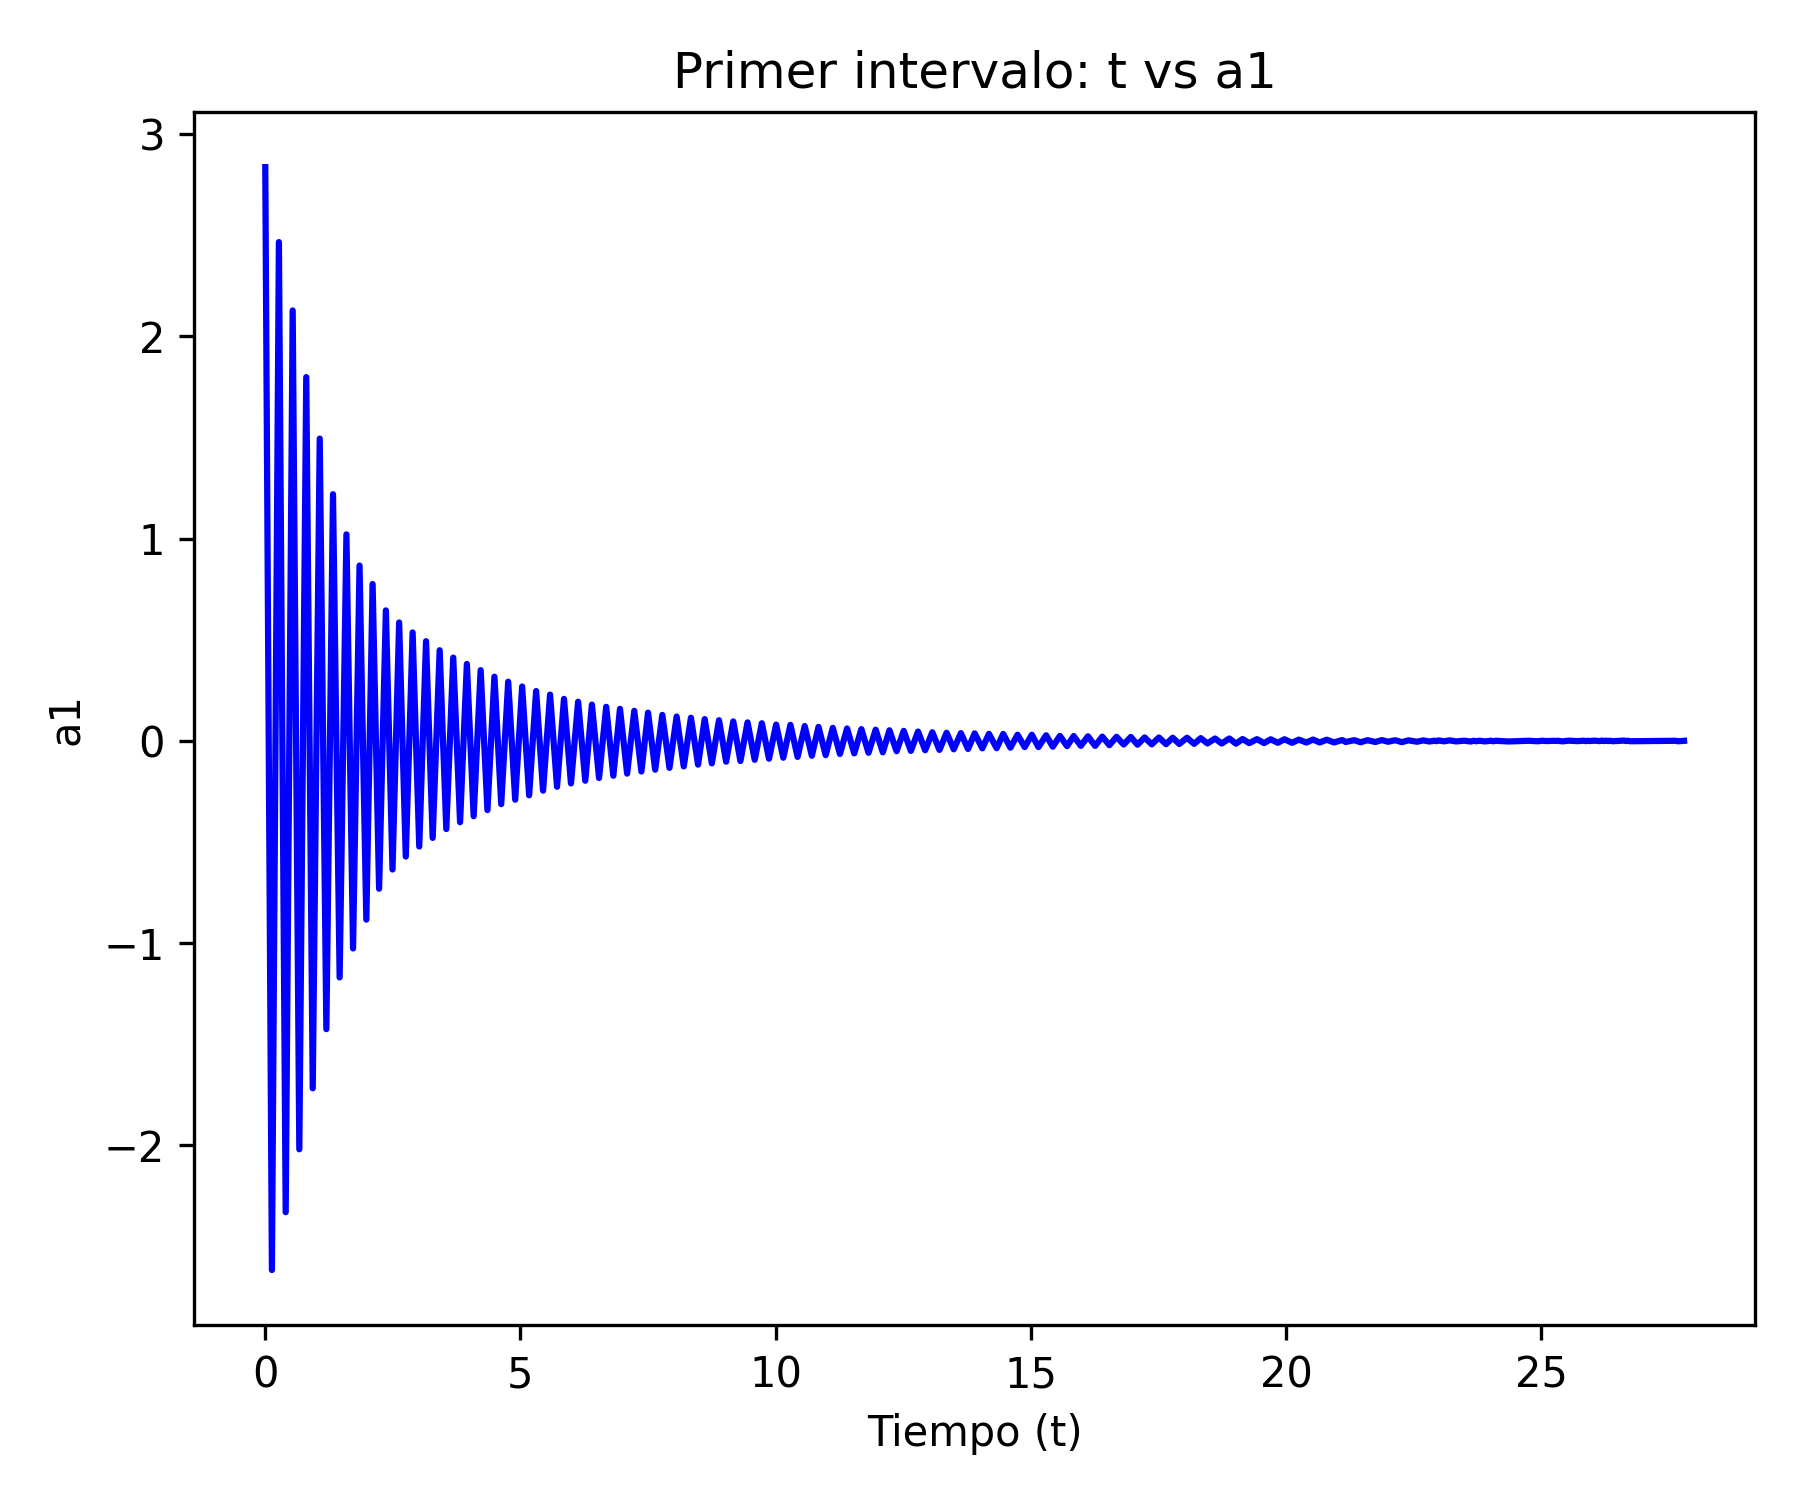
\includegraphics[width=0.5\textwidth]{GRAFICOS/pullback_first.png}
  \caption{Filtered signal of the pull-back test of system 1.}
  \label{fig:filtered_signal1}
\end{figure}

\begin{figure}[h]
  \centering
  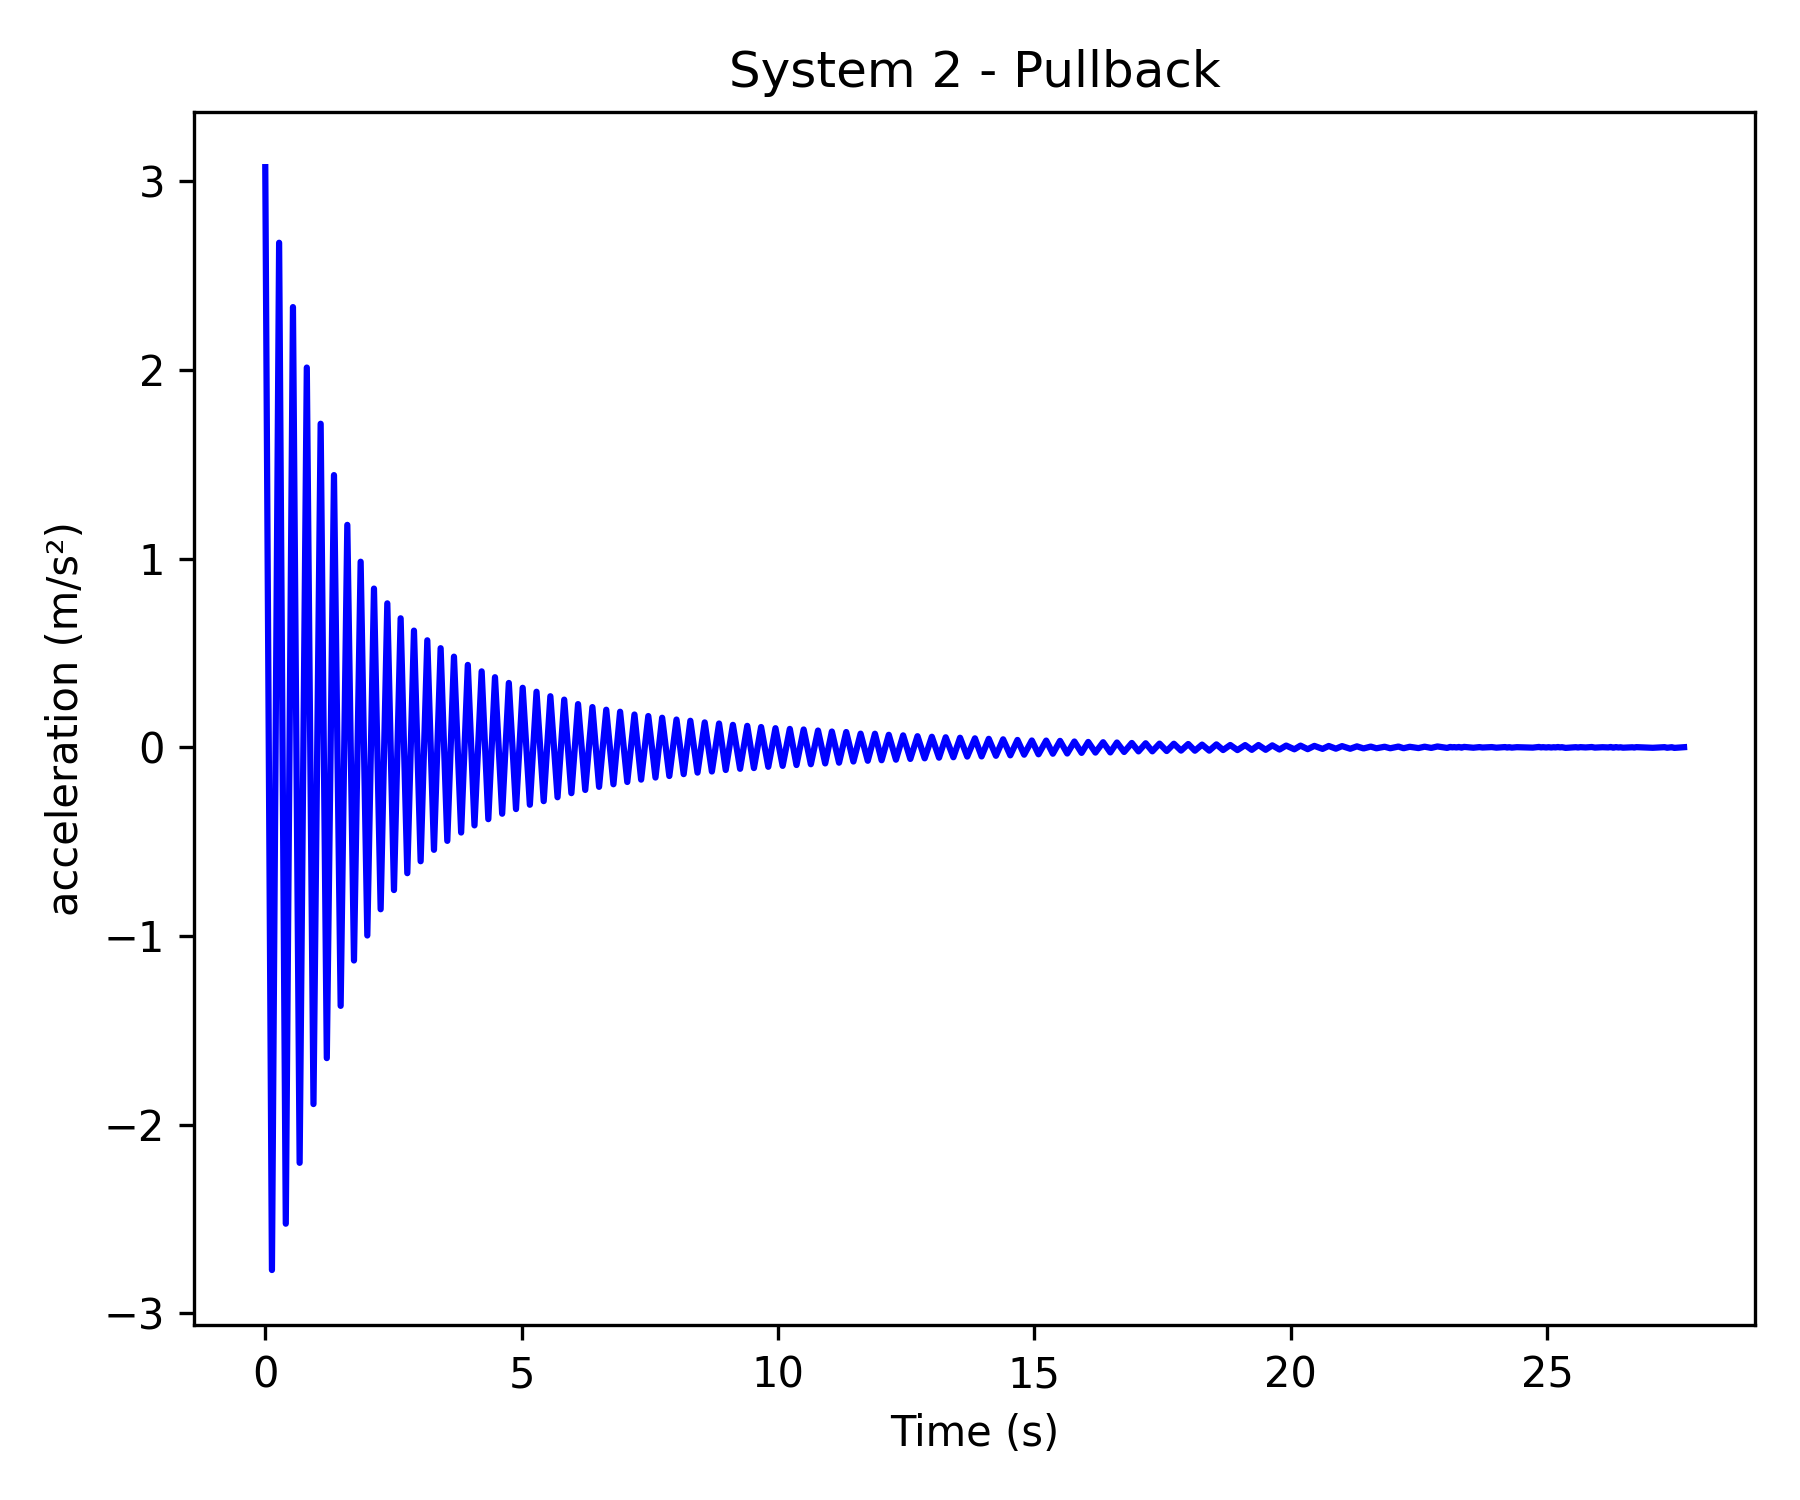
\includegraphics[width=0.5\textwidth]{GRAFICOS/pullback_second.png}
  \caption{Filtered signal of the pull-back test of system 1.}
  \label{fig:filtered_signal2}
\end{figure}

With the filtered signal, we can start the analysis of the systems.

\subsection{Pull-back Test}
\subsubsection{Determination of the damping period, natural period and damping ratio}
To determine the period of the systems, we used the logarithmic decrement method. This method is based on the analysis of the acceleration signal obtained from the accelerometer during the pull-back test. The logarithmic decrement is calculated using equation (\ref{eq:log_dec}).\\
First, we analysed the acceleration signal obtained from the system without damping (system 1). The signal was detrended and filtered to remove unwanted components. After that, we calculated the logarithmic decrement and plotted the results that are shown in Figure~\ref{fig:pullback1}.



\begin{figure}[h]
  \centering
  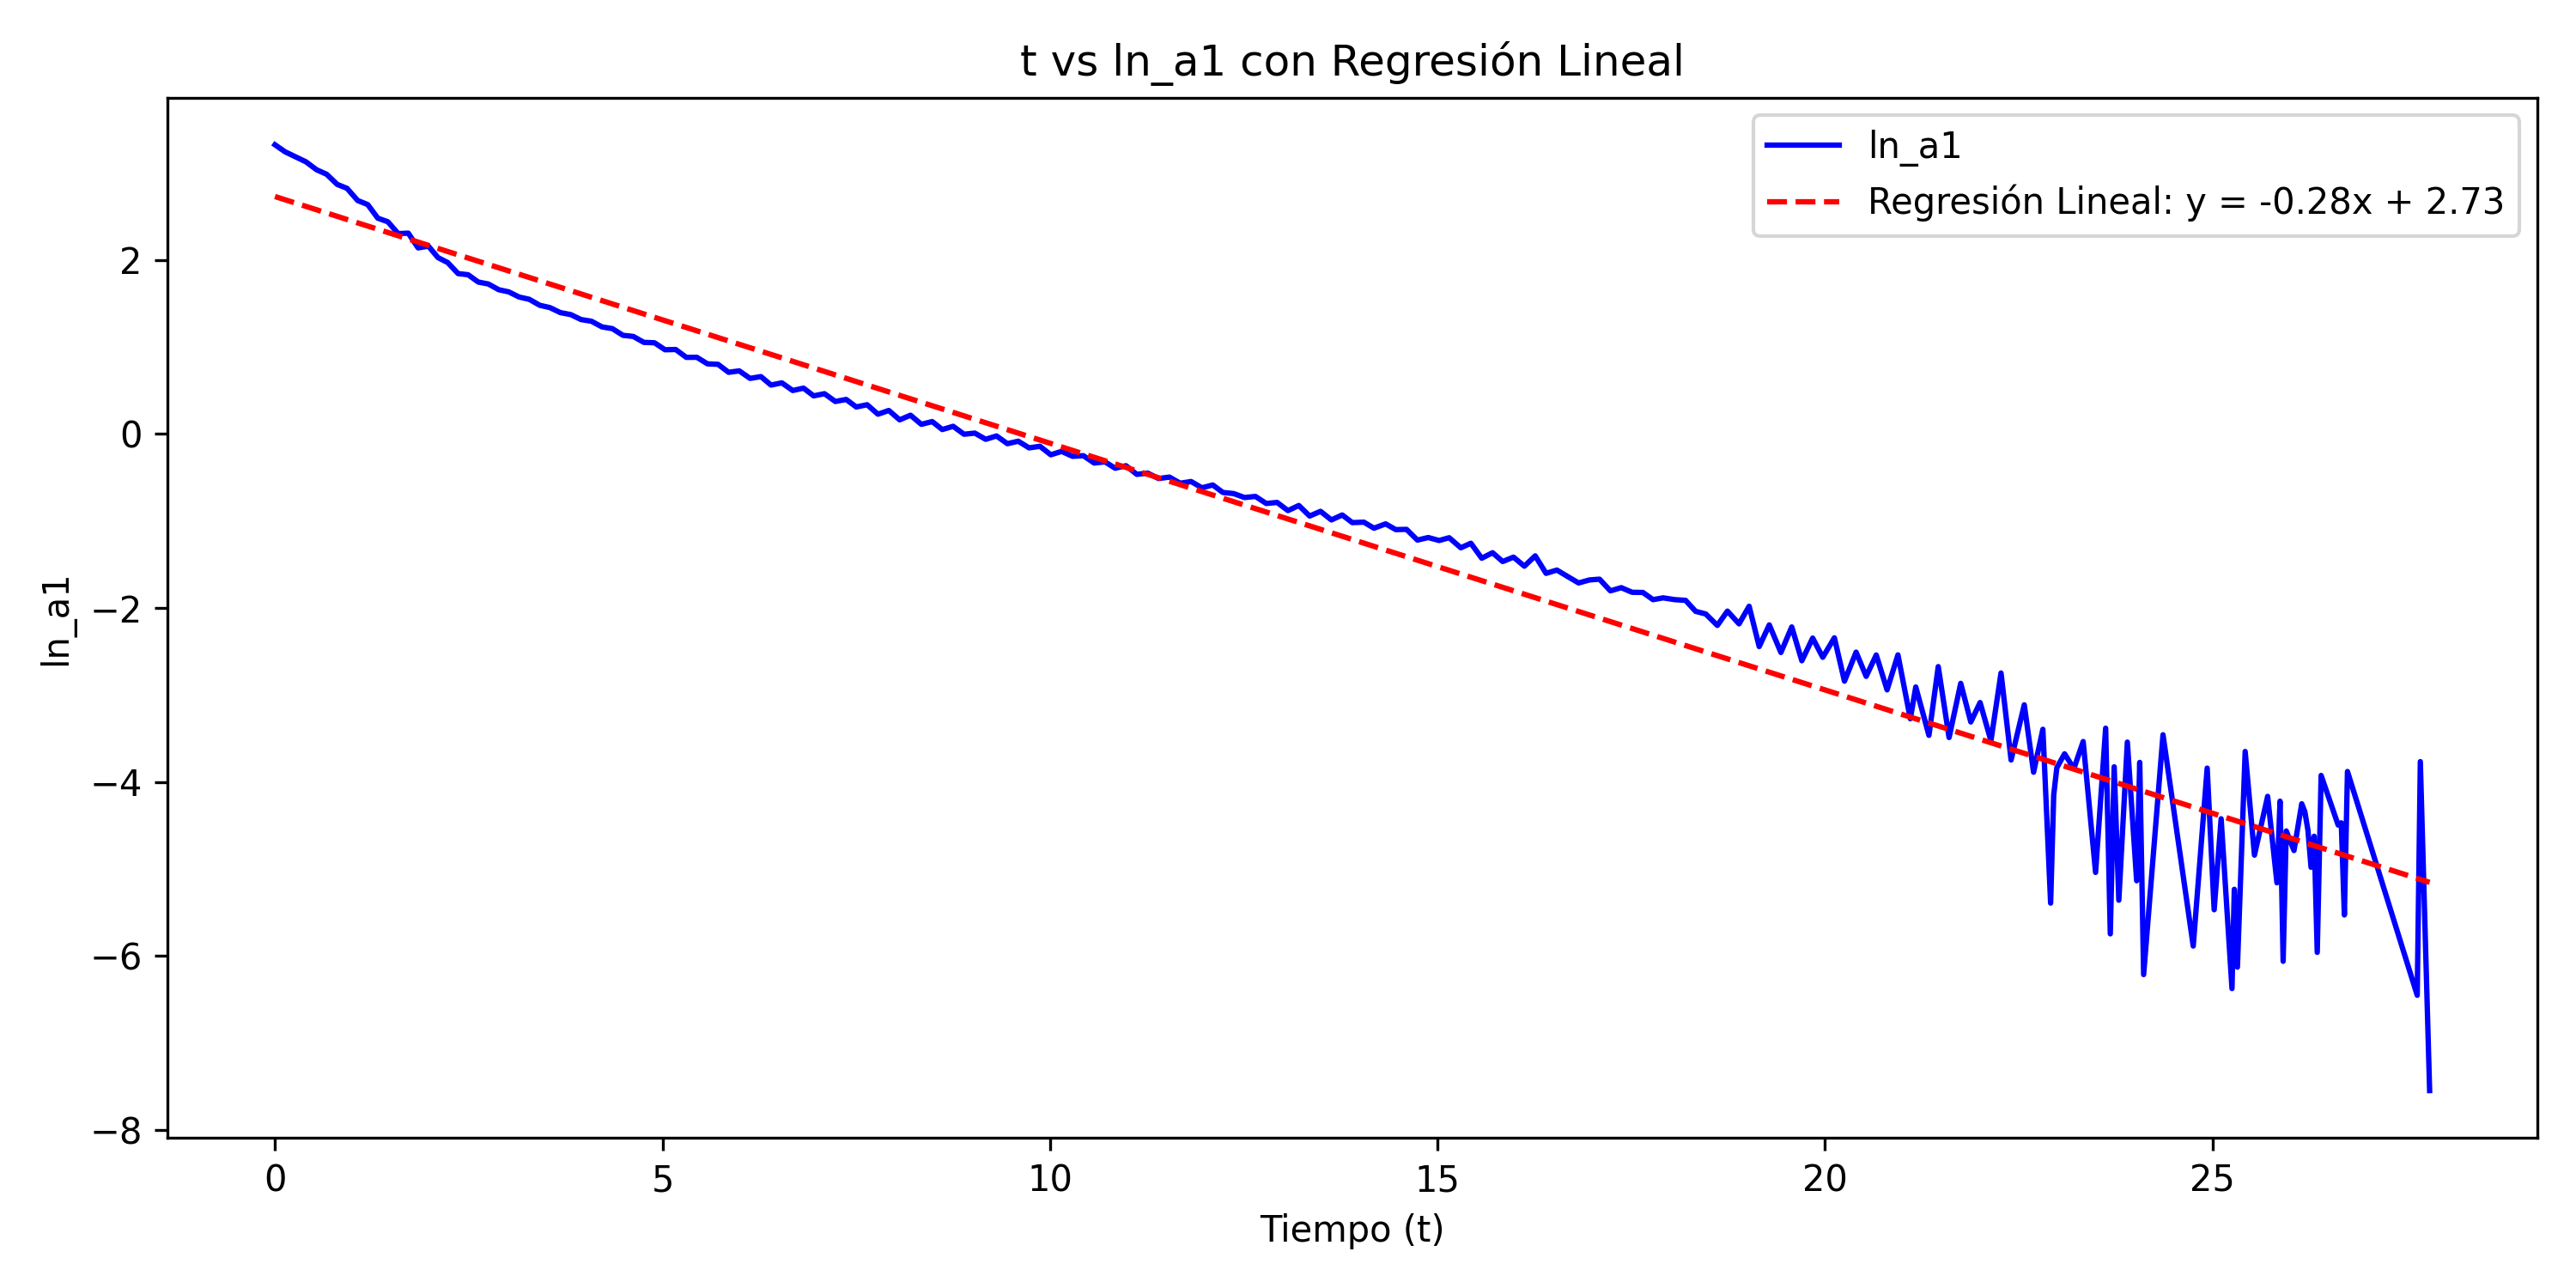
\includegraphics[width=0.8\textwidth]{GRAFICOS/regresion_lineal_first.png}
  \caption{Logarithmic decrement of the pull-back test.}
  \label{fig:pullback1}  
\end{figure}

Then, we analysed the acceleration signal obtained from the system with damping (system 2). The signal was detrended and filtered to remove unwanted components. The resulting signal is shown in Figure~\ref{fig:pullback2}.

\begin{figure}[h]
  \centering
  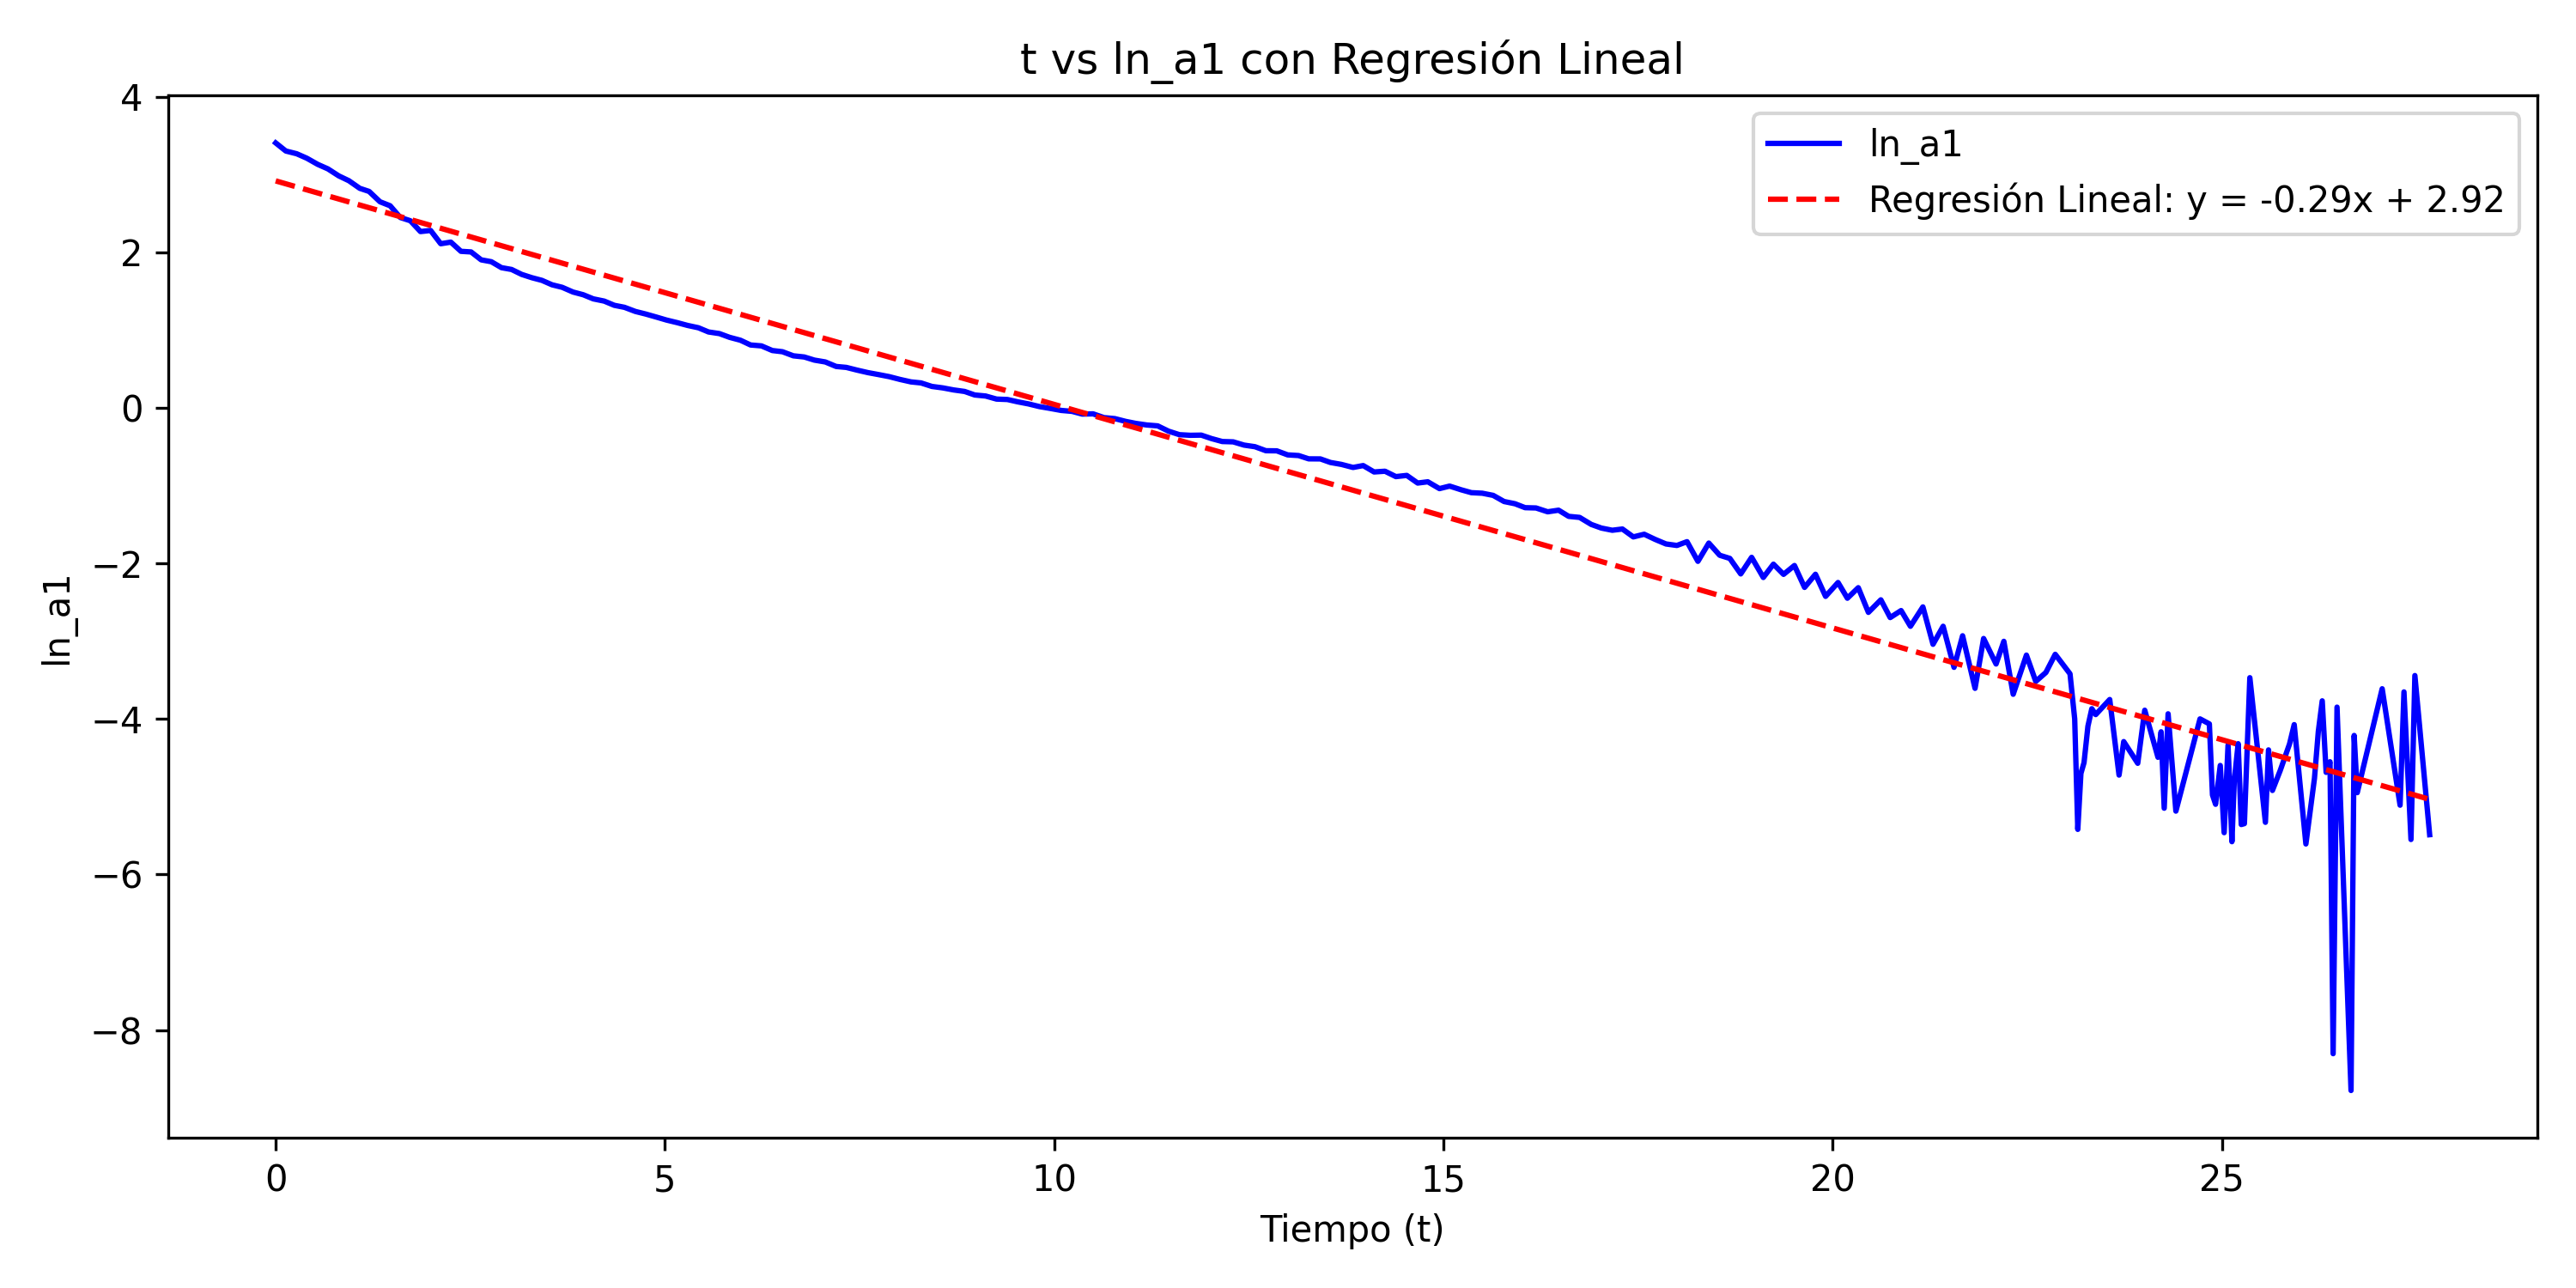
\includegraphics[width=0.8\textwidth]{GRAFICOS/regresion_lineal_second.png}
  \caption{Logarithmic decrement of the pull-back test.}
  \label{fig:pullback2}  
\end{figure}

\newpage

\begin{table}[h]
\centering
  \begin{tabular}{|c|c|c|}
  \hline
  \textbf{Item}& \textbf{System 1}& \textbf{System 2} \\ \hline
  \textbf{$\omega_n$(rad/s)} & 23.96 & 25.2  \\ \hline
  \textbf{Natural Period (s)} & 0.262246& 0.249264  \\ \hline
  \textbf{Damping ratio} & 0.0118&0.0114  \\ \hline
  \textbf{Damping Period(s)} & 0.262282&0.249296  \\ \hline
  \end{tabular}
\caption{Natural period, Dumping period and damping ratio from logarithmic decrement of the pull-back test.}
\label{tab:pullback}
\end{table}

As shown in Table~\ref{tab:pullback}, the natural period of the system without damping (system 1) is 0.262246 s, is slightly higher than the natural period of the system with damping (system 2), which is 0.249264 s. This is expected, as the presence of damping reduces the natural frequency of the system.\\

Figures~\ref{fig:pullback1} and~\ref{fig:pullback2} display the natural logarithm of acceleration versus time for Systems 1 and 2, respectively. For System 1, the regression line shows a slope of approximately $-0.28$, while for System 2 the slope is about $-0.29$. These results are consistent with the damping ratios previously calculated using the system's natural frequencies. Both systems exhibit very low damping, confirming that they behave as lightly damped single-degree-of-freedom systems. The linear trend of the logarithmic amplitude also supports the assumption of linear damping in the analysis.

\subsection{Test with harmonic vibration at the base of varying frequencies}

In this section, the natural frequency and damping ratio were adjusted so that the transmissibility function  fits the experimental data. The algorithm took as initial parameters the natural frequency and damping ratio obtained from the pull-back test. The transmissibility function was calculated using equation (\ref{eq:transmissibility}).

The results are shown below:

\begin{figure}[H]
  \centering
  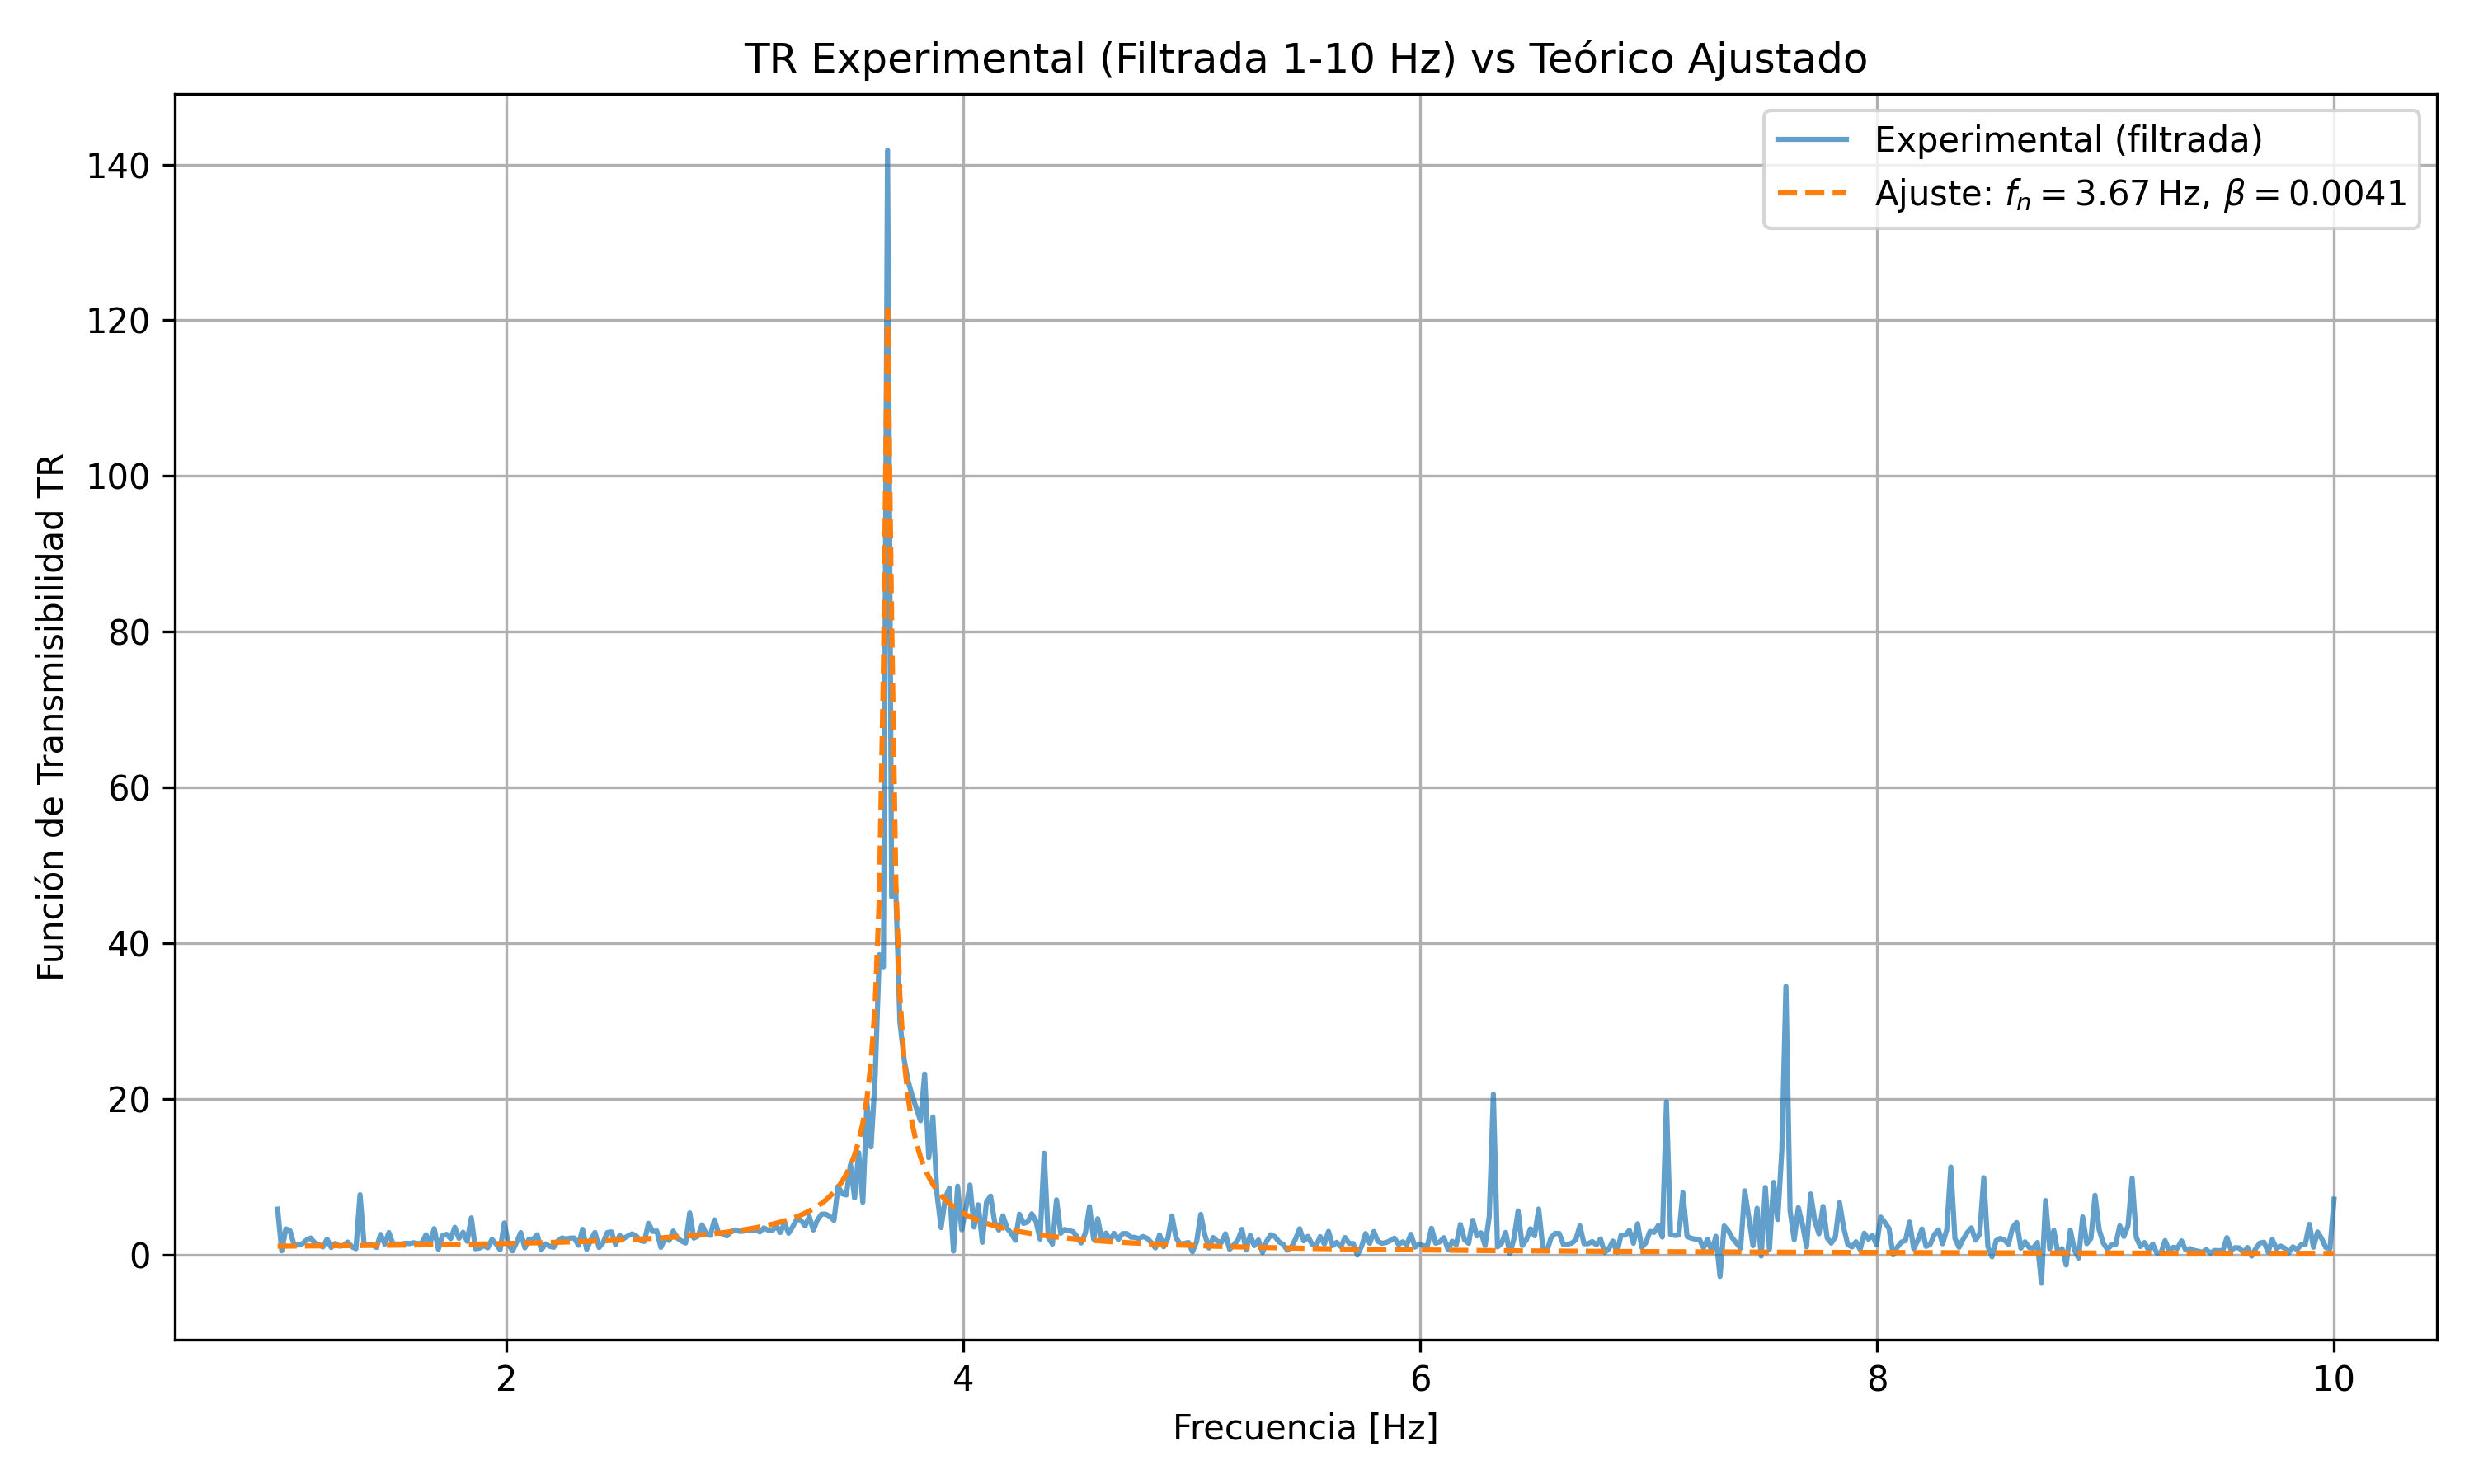
\includegraphics[width=0.8\textwidth]{GRAFICOS/TR_vs_teorico.png}
  \caption{Transmissibility function - Experimental vs Theoretical.}
  \label{fig:transmissibility}
\end{figure}

For better visualization, de frequency data was filtered between 1 - 10 Hz and the adjusted parameters for the function to fit the experimental data were:

\begin{table}[H]
\centering
\caption{Adjusted parameters for the transmissibility function.}
\begin{tabular}{|c|c|}
\hline
\textbf{Parameter} & \textbf{Value} \\ \hline
Natural Frequency ($f_n$) & 3.67 Hz \\ \hline
Damping Ratio ($\beta$) & 0.0041 \\ \hline
\end{tabular}
\end{table}

\subsection{Seismic Response}

This section presents the result of the sismic response of the structure due to the Concepcion and Kobe earthquakes. The following results were obtained by using the Newmark method.

\begin{figure}[H]
  \centering
  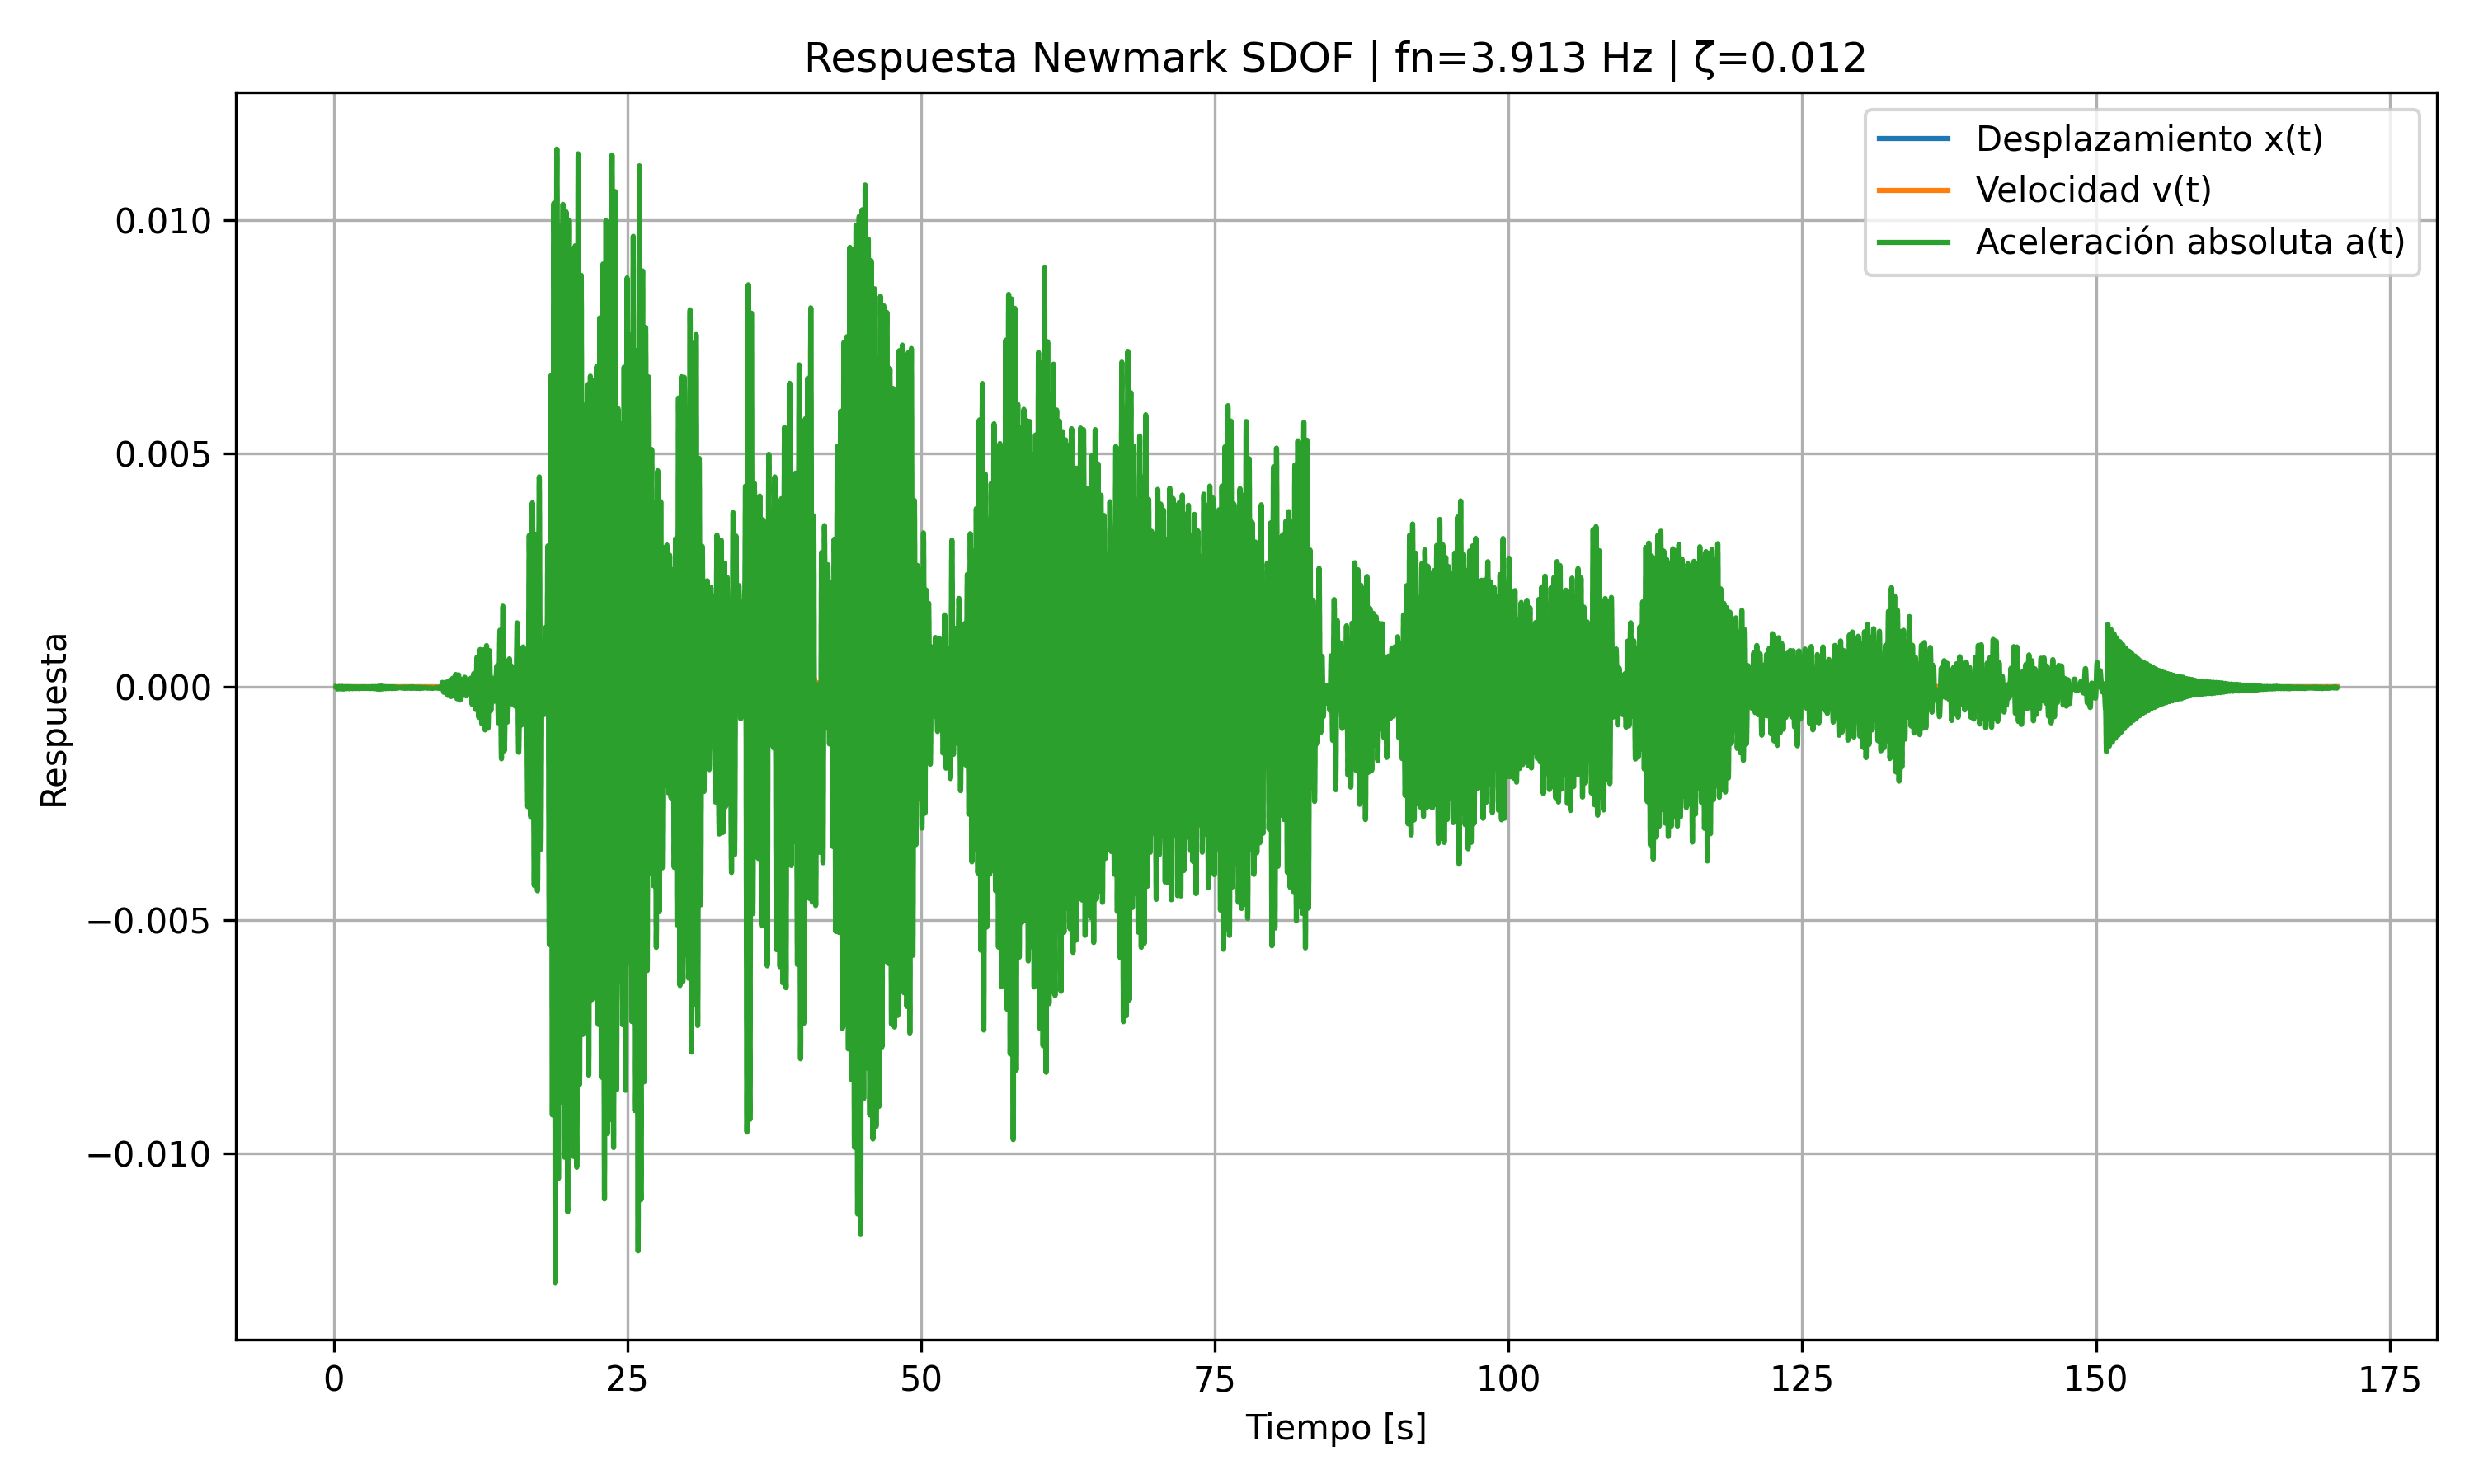
\includegraphics[width=0.8\textwidth]{GRAFICOS/respnewmark_Concepcion.png}
  \caption{Concepcion Earthquake - Seismic Response.}
  \label{fig:concepcion}
\end{figure}

\begin{figure}[H]
  \centering
  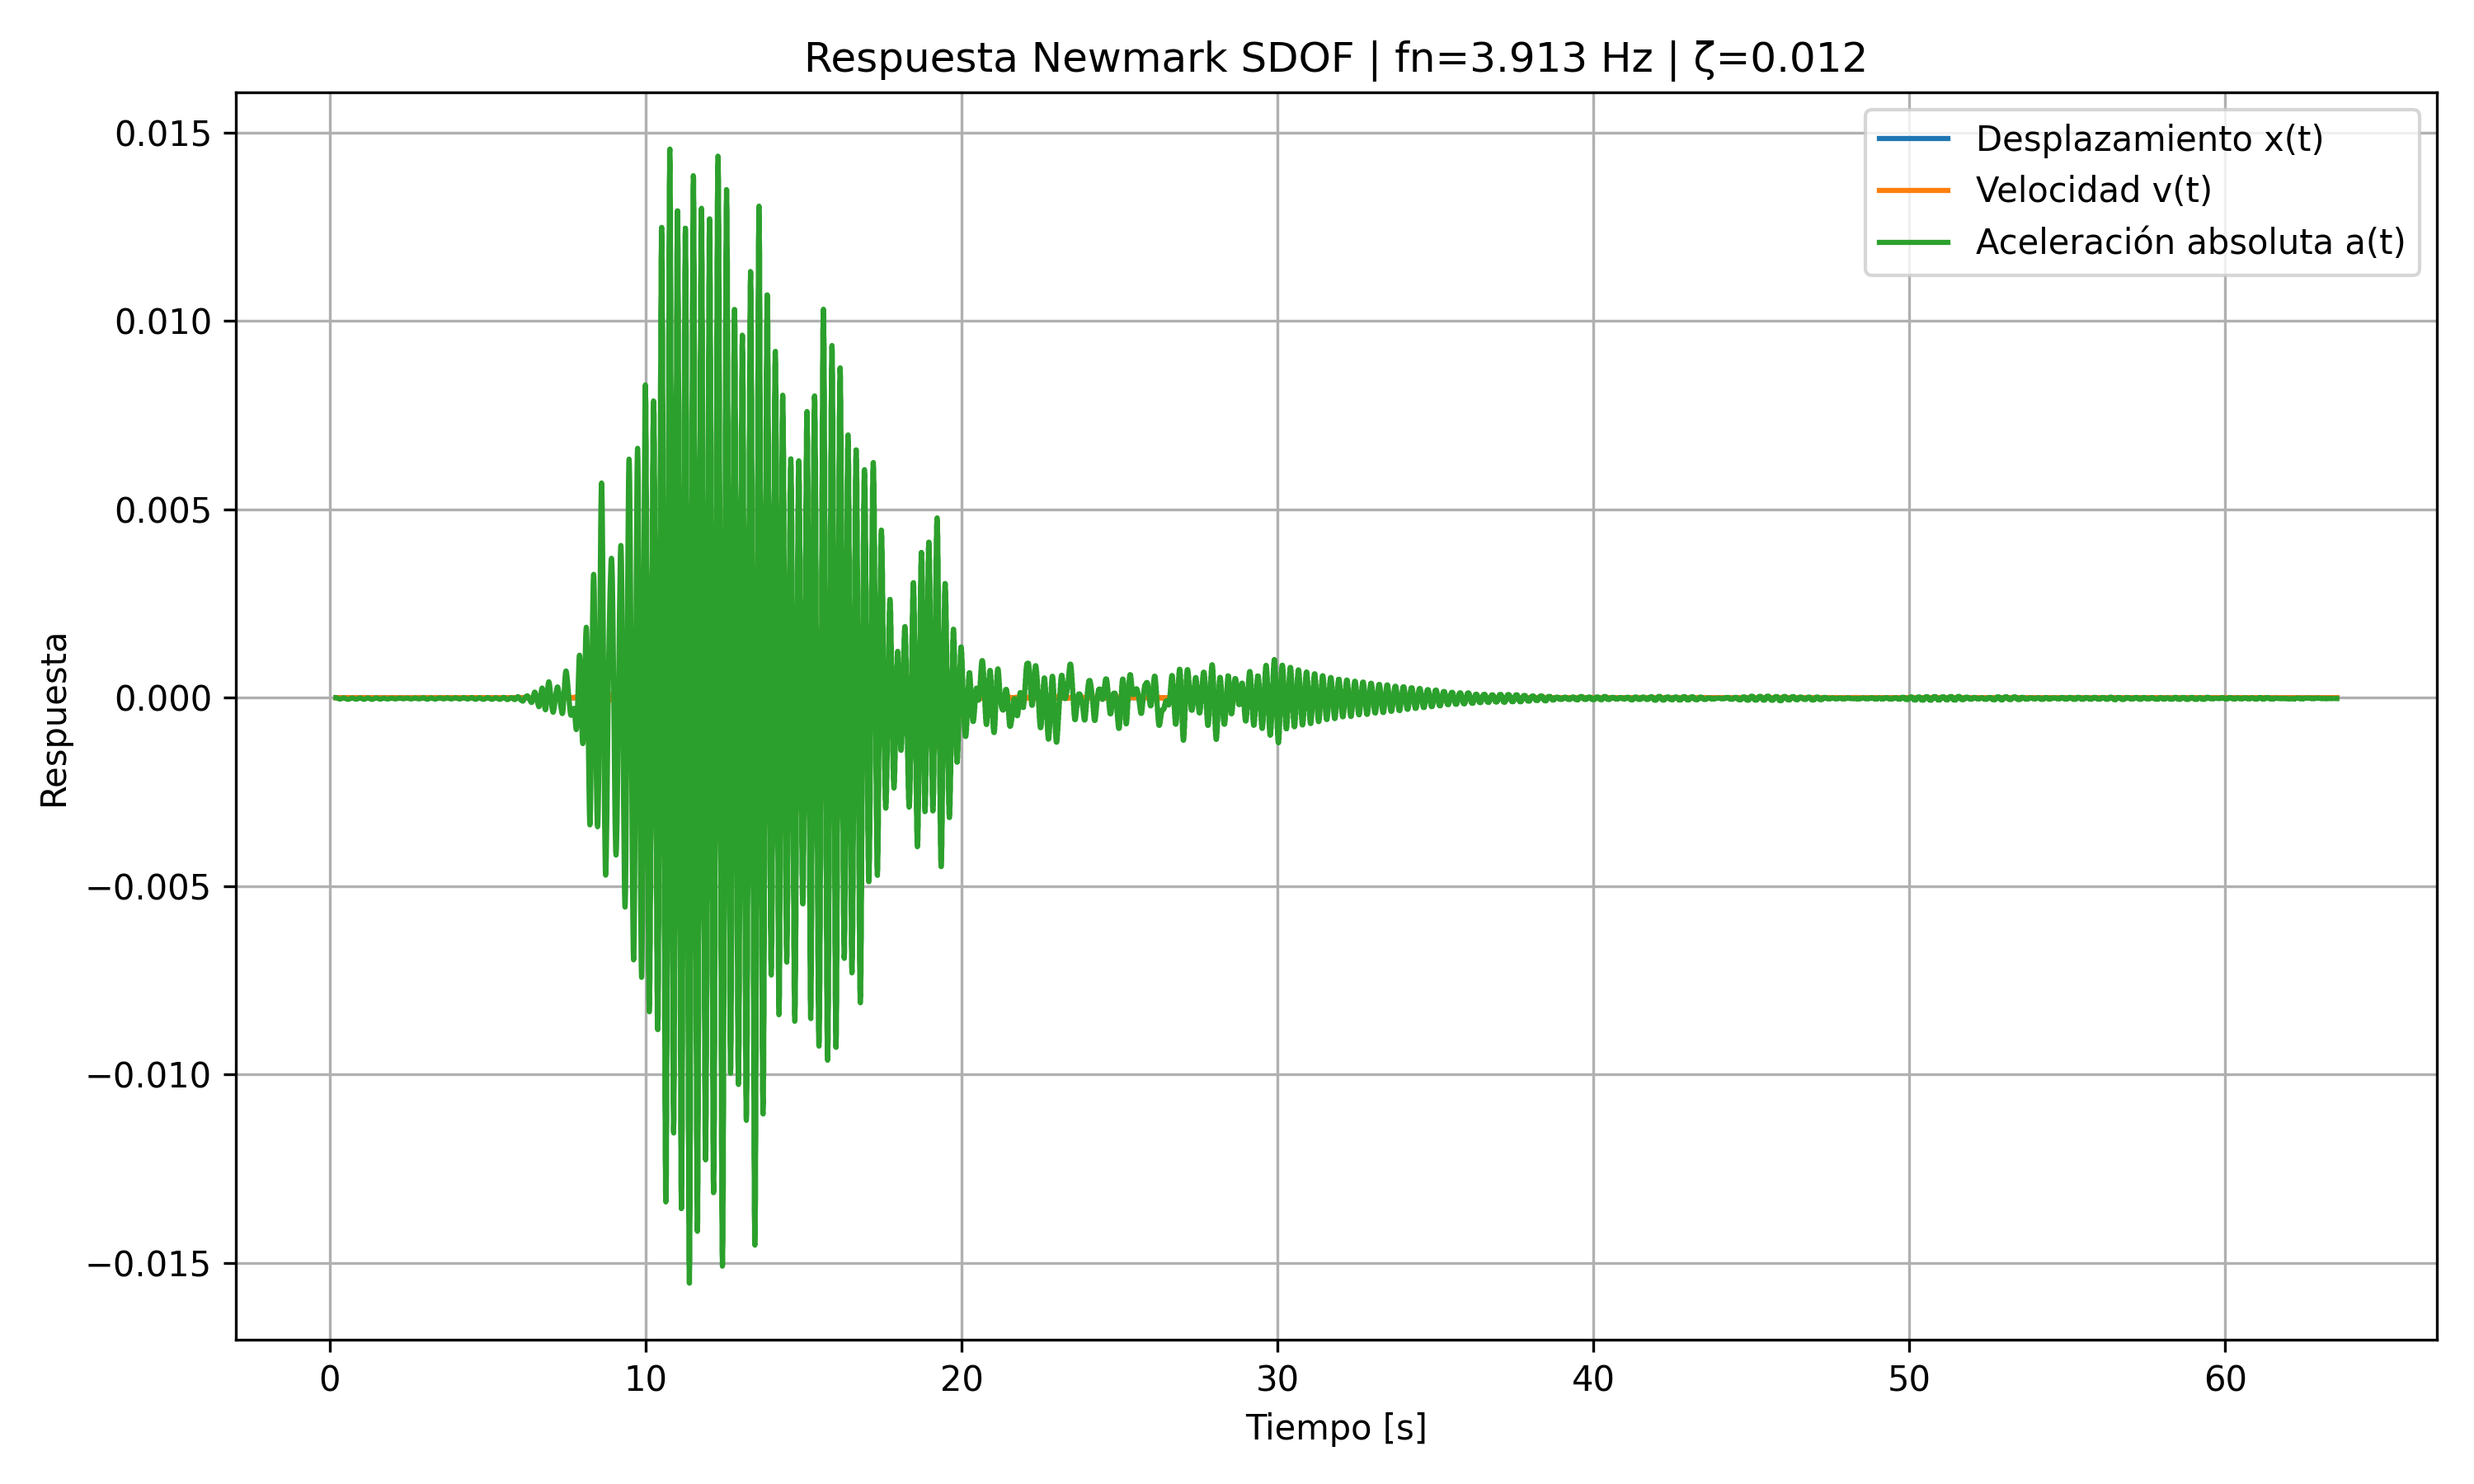
\includegraphics[width=0.8\textwidth]{GRAFICOS/respnewmark_Kobe.png}
  \caption{Kobe Earthquake - Seismic Response.}
  \label{fig:kobe}
\end{figure}

\subsection{Transfer Function}

The transfer function is a mathematical representation of the relationship between the input and output of a system in the frequency domain. It is defined as the ratio of the output response to the input response, and it can be calculated using the following formula:

\begin{equation}
  H(\omega) = \frac{\ddot{u}}{\ddot{u_g}} = \frac{X}{U}
\end{equation}

Where:
\begin{itemize}
  \item $H(\omega)$ = transfer function (dimensionless)
  \item $\ddot{u_g}$ = output acceleration (m/s$^2$) (acceleration of the base) 
  \item $\ddot{u}$ = input acceleration (m/s$^2$) (acceleration of the mass)
  \item $X$ = output response (m/s$^2$)
  \item $U$ = input response (m/s$^2$)
\end{itemize}

In this section the transfer function of the total acceleration and the base acceleration was determined, as well as an estimated natural frequency. The results are shown below:

\begin{figure}[H]
  \centering
  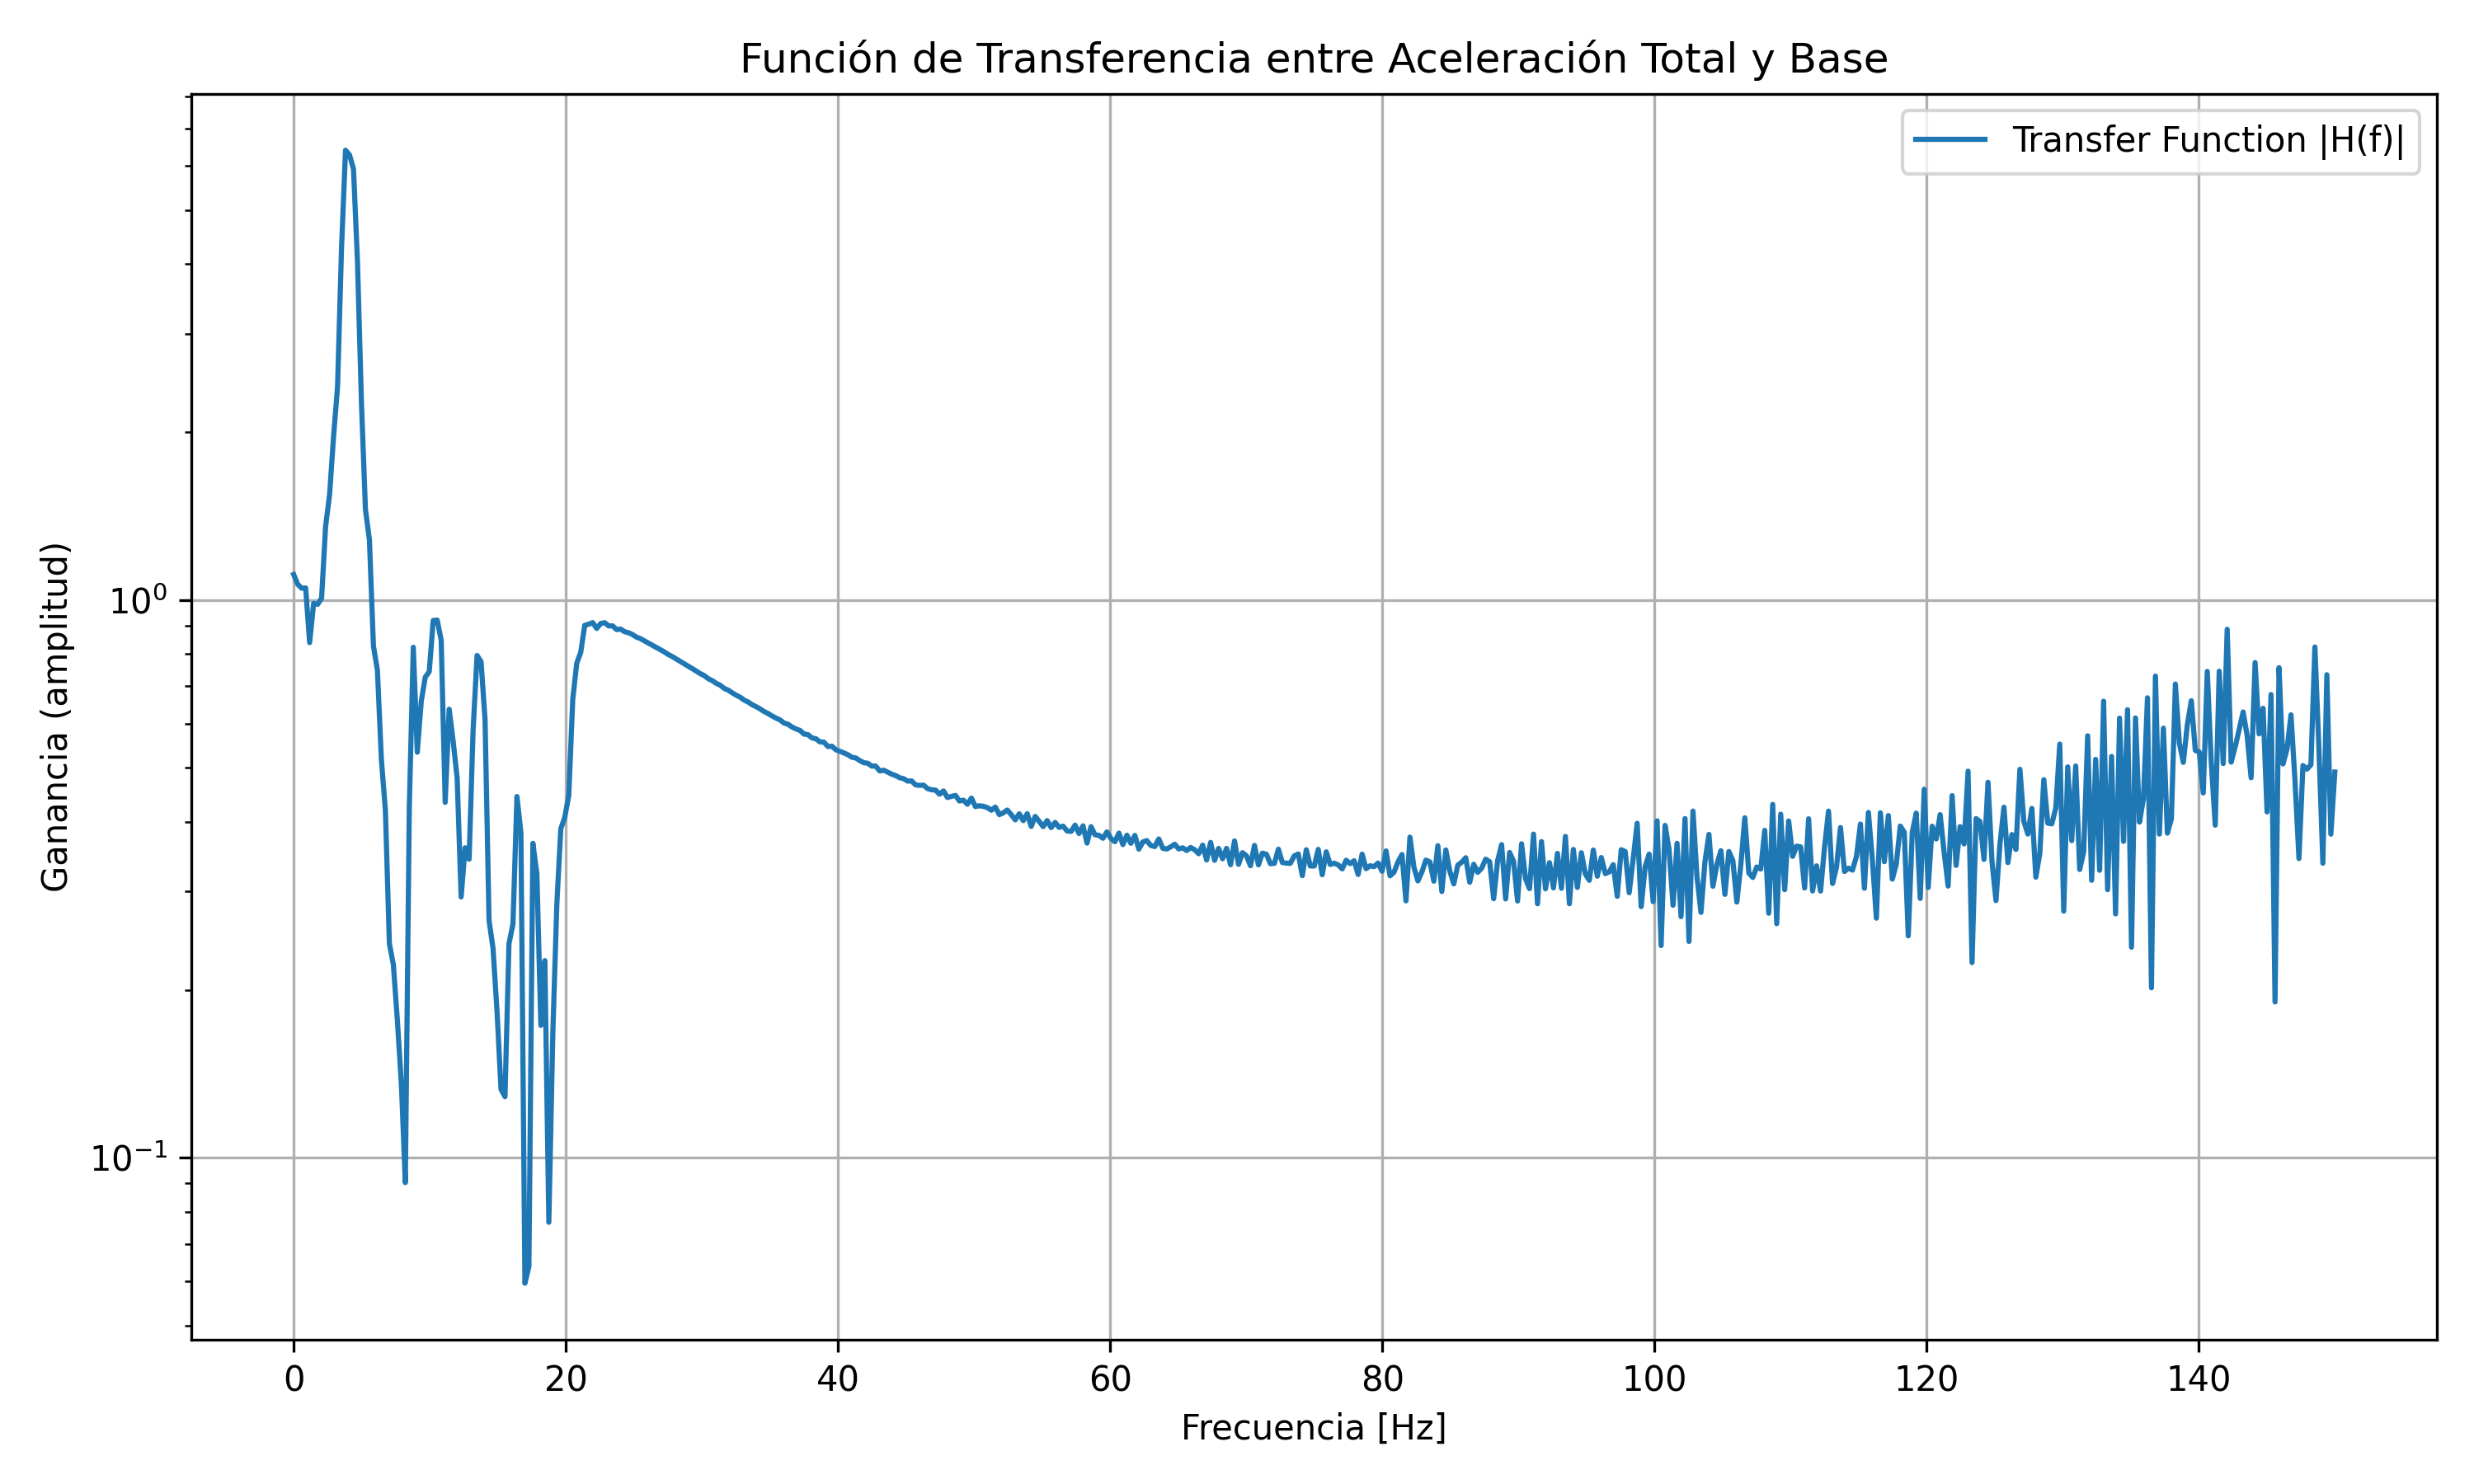
\includegraphics[width=0.8\textwidth]{GRAFICOS/TransferFunction_TFEstimate.png}
  \caption{Transfer Function - Total Acceleration vs Base Acceleration of the Concepcion Earthquake.}
  \label{fig:transfer}
\end{figure}

\begin{figure}[H]
  \centering
  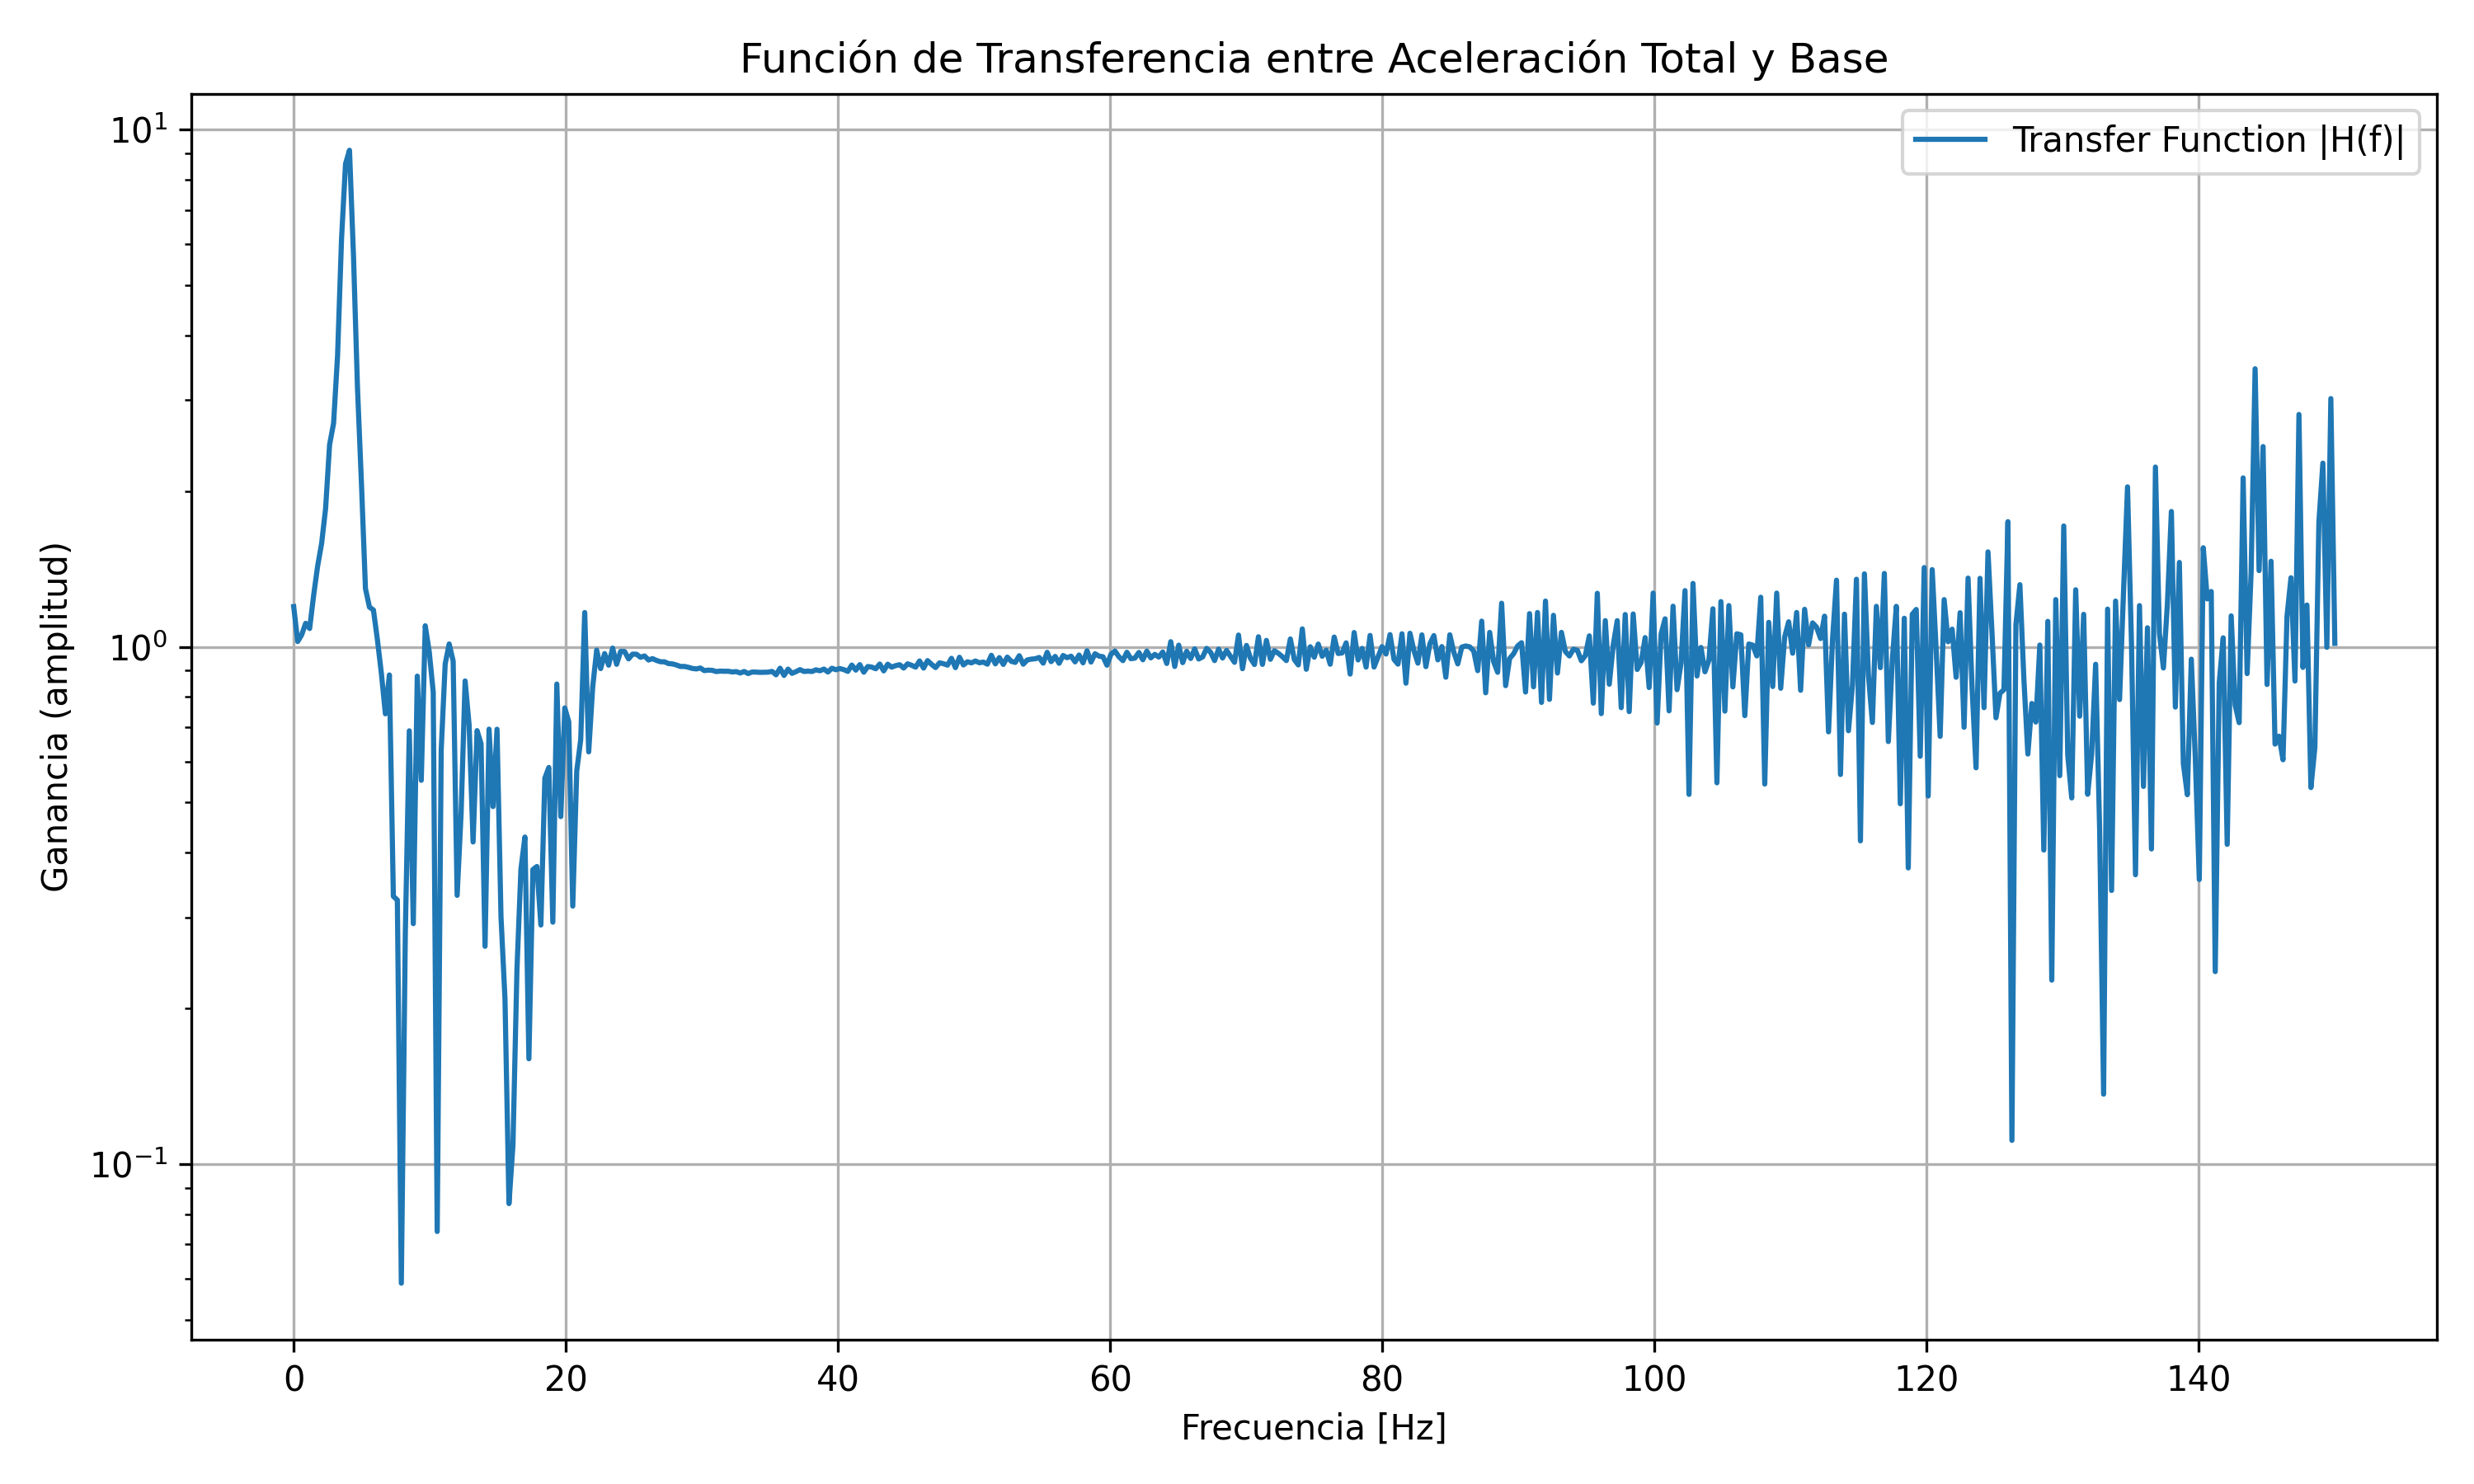
\includegraphics[width=0.8\textwidth]{GRAFICOS/TransferFunction_TFEstimate_Kobe.png}
  \caption{Transfer Function - Total Acceleration vs Base Acceleration of the Kobe Earthquake.}
  \label{fig:transfer_kobe}
\end{figure}

The estimated natural frequencies of both earthquakes are shown in the table below:

\begin{table}[H]
\centering
\caption{Estimated natural frequencies of the earthquakes.}
\begin{tabular}{|c|c|}
\hline
\textbf{Earthquake} & \textbf{Natural Frequency (Hz)} \\ \hline
Concepcion & 3.81 \\ \hline
Kobe & 4.10 \\ \hline
\end{tabular}
\end{table}


\newpage
\section{Discussion}
\subsection{Theoretical vs Experimental Results}

The results from the pull-back test were compared to theoretical values calculated using the system's mass and stiffness. The natural frequency and period were obtained analytically, while the damping ratio was estimated experimentally using the logarithmic decrement method.

As shown in Table~\ref{tab:results}, the experimental natural frequency and period differ from the theoretical values by approximately 12.3\% and 11\%, respectively. These differences may be due to modeling simplifications or experimental uncertainties. The measured damping ratio confirms that the system is lightly damped.

\begin{table}[h]
\centering
\begin{tabular}{|c|c|c|c|}
\hline
\textbf{Parameter} & \textbf{Theoretical} & \textbf{Experimental} & \textbf{Error (\%)} \\ \hline
Natural frequency $\omega_n$ (rad/s) & 26.9 & 23.96 & 12.3\% \\ \hline
Natural period $T_n$ (s) & 0.233 & 0.262 & 11.0\% \\ \hline
Damping ratio $\zeta$ & 0 & 0.0118 & -- \\ \hline
\end{tabular}
\caption{Comparison between theoretical and experimental values of natural frequency, period, and damping ratio.}
\label{tab:results}
\end{table}

\subsection{Comparison of Dynamic Properties from Different Tests}

Dynamic properties obtained from the pull-back test, harmonic excitation, and transfer function analysis were generally consistent, though slight differences were observed. The pull-back test yielded a natural frequency of 23.96~rad/s, while frequency-domain methods gave slightly lower values due to damping and processing effects. Damping ratios ranged from 0.0041 to 0.0118. Each method emphasized different aspects of system behavior, highlighting the influence of test conditions and input type.

\subsection{Sources of Error and Improvement Suggestions}

Discrepancies between theoretical and experimental results arise from modeling simplifications, such as idealized boundary conditions and neglected damping sources, as well as experimental factors like sensor noise and signal filtering. Variations in natural frequencies and damping ratios across tests highlight these limitations.

To improve accuracy, future tests could use higher-resolution sensors, better mounting stability, and increased sampling rates. Additionally, repeating tests and validating results with numerical models would help enhance reliability.

\newpage

\section{Conclusions}

The laboratory validated several key concepts introduced in lectures. The natural frequency and damping ratio of an SDOF system were successfully identified using the pull-back test and logarithmic decrement method, confirming the theoretical relationships between mass, stiffness, and frequency. The resonance phenomenon was clearly observed during harmonic base excitation, aligning with the predicted amplification at the system’s natural frequency. The transmissibility function and transfer function analysis also supported the expected frequency-dependent response behavior. Overall, the experiment demonstrated how theoretical dynamic models can accurately describe the real behavior of lightly damped systems.

\newpage

\nocite{*}
\bibliography{referencias}

\end{document} 